\documentclass[letterpaper,12pt]{article}
\usepackage[utf8]{inputenc}
\usepackage[spanish]{babel}
\usepackage{graphicx}
\usepackage{amsmath}
\usepackage{amssymb}
\usepackage[margin=0.75in]{geometry}
\usepackage{chngcntr}
\usepackage{caption}
\usepackage{fancyhdr}
\usepackage{placeins}

% Ajustar la altura del encabezado
\setlength{\headheight}{14.5pt}
\addtolength{\topmargin}{2.5pt}
\setlength{\parskip}{1em}

% Configurar la numeración de secciones y subsecciones
\renewcommand{\thesection}{14.\arabic{section}}
\renewcommand{\thesubsection}{14.\arabic{section}.\arabic{subsection}}

% Redefinir el contador de figuras
\captionsetup[figure]{labelformat=empty} % Evitar la numeración automática
\captionsetup[table]{labelformat=empty} % Evitar la numeración automática

% Configurar fancyhdr
\pagestyle{fancy}
\fancyhf{}
\fancyhead[L]{Capítulo 14}
\fancyhead[R]{\thepage}
\fancyfoot[C]{}

\title{Esquemas Avanzados de Control de Drive}
\author{}
\date{}

\begin{document}

\maketitle
\thispagestyle{fancy} % Aplicar el estilo fancyhdr a la primera página

\section{Introducción}

Dos esquemas de control avanzados, el control orientado al campo (FOC) y el control directo de par (DTC), se han convertido en los estándares industriales en drives de media tensión (MV) de alta potencia. Esto se debe a lo siguiente: (a) Los esquemas de control ofrecen un rendimiento dinámico superior; (b) sus algoritmos pueden implementarse eficientemente en tiempo real mediante procesadores digitales; y (c) la diferencia de costo entre las implementaciones digitales de esquemas de control avanzados y de bajo rendimiento es mínima.

Este capítulo se centra en los esquemas FOC y DTC para drives de motores de inducción. Comienza con una introducción a la transformación del marco de referencia, seguida de modelos dinámicos del motor de inducción. Se presentan varios esquemas de control orientados al campo para los drives de fuente de voltaje y corriente. El énfasis está en el esquema de control orientado al flujo del rotor debido a su simplicidad y amplia aceptación en los drives de MV. También se elabora sobre el control directo de par. Los conceptos importantes se ilustran con simulaciones por computadora y experimentos. El capítulo finaliza con una comparación entre los esquemas FOC y DTC.

\section{Transformación del Marco de Referencia}

El uso de la teoría del marco de referencia puede simplificar el análisis de las máquinas eléctricas y también proporcionar una herramienta poderosa para la implementación digital de esquemas de control sofisticados para los drives de corriente alterna. Se han propuesto varios marcos de referencia a lo largo de los años [1], de los cuales los marcos de referencia estacionario y síncrono son los más comúnmente utilizados. A continuación, se presenta la transformación de variables entre los dos marcos.

\clearpage
\subsection{Transformación de Marco abc/dq}

La transformación de las variables trifásicas (eje abc) de un motor de inducción a las variables bifásicas equivalentes (eje dq) puede realizarse mediante

\begin{equation}
\begin{bmatrix}
x_d \\
x_q
\end{bmatrix}
=
\frac{2}{3}
\begin{bmatrix}
\cos \theta & \cos(\theta - 2\pi/3) & \cos(\theta - 4\pi/3) \\
-\sin \theta & -\sin(\theta - 2\pi/3) & -\sin(\theta - 4\pi/3)
\end{bmatrix}
\begin{bmatrix}
x_a \\
x_b \\
x_c
\end{bmatrix} \tag{14.2-1}
\end{equation}

donde $x$ representa ya sea corriente, voltaje o enlace de flujo, y $\theta$ es el desplazamiento angular entre el eje a y el eje d de los marcos de referencia trifásico y bifásico como se muestra en la Fig. 14.2-1. Las variables trifásicas, $x_a, x_b$ y $x_c$, están en el \textit{marco de referencia estacionario} que no rota en el espacio, mientras que las variables bifásicas, $x_d$ y $x_q$, están en el \textit{marco de referencia síncrono} cuyos ejes directo (d) y en cuadratura (q) rotan en el espacio a la velocidad síncrona $\omega_e$. Cabe señalar que $\omega_e$ es la velocidad angular eléctrica (no mecánica) del campo magnético rotatorio del motor, dada por

\begin{equation}
\omega_e = 2 \pi f_s \tag{14.2-2}
\end{equation}

donde $f_s$ es la frecuencia de las variables del estator. El ángulo $\theta$ se puede encontrar a partir de

\begin{equation}
\theta(t) = \int_{0}^{t} \omega_e(t) dt + \theta_0 \tag{14.2-3}
\end{equation}

\begin{figure}[ht]
\centering
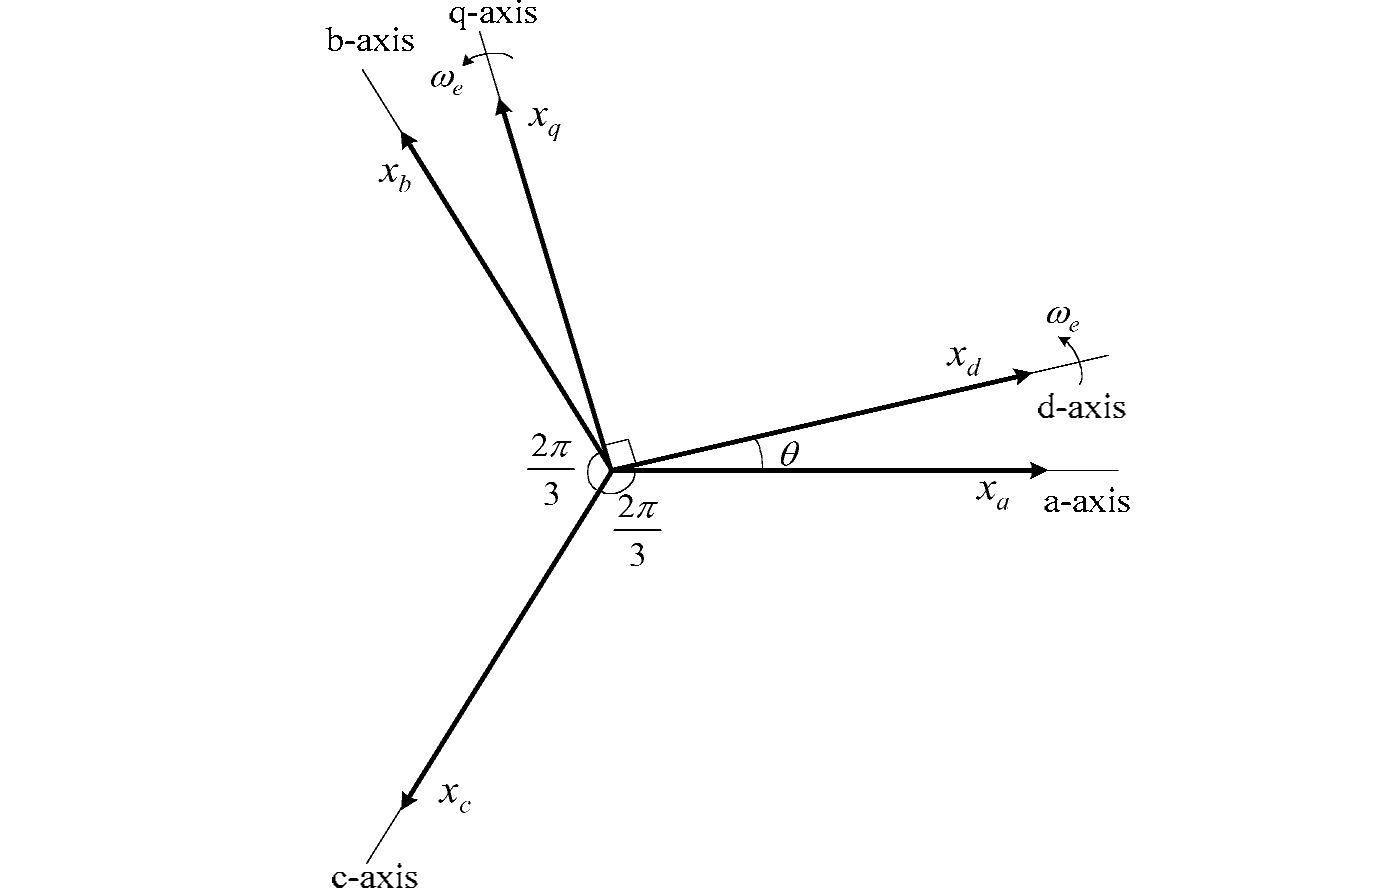
\includegraphics{graficos/img01.jpg}
\caption{Figura 14.2-1: Variables en el marco trifásico (abc) estacionario y en el marco bifásico (dq) síncrono.}
\end{figure}
\FloatBarrier

\clearpage
Cabe señalar que la ecuación de transformación (14.2-1) es válida solo para un sistema trifásico balanceado, en el cual

\begin{equation}
x_a + x_b + x_c = 0 \tag{14.2-4}
\end{equation}

De manera similar, las variables bifásicas en el marco síncrono pueden transformarse nuevamente al marco trifásico estacionario mediante

\begin{equation}
\begin{bmatrix}
x_a \\
x_b \\
x_c
\end{bmatrix}
=
\begin{bmatrix}
\cos \theta & -\sin \theta \\
\cos(\theta - 2\pi/3) & -\sin(\theta - 2\pi/3) \\
\cos(\theta - 4\pi/3) & -\sin(\theta - 4\pi/3)
\end{bmatrix}
\begin{bmatrix}
x_d \\
x_q
\end{bmatrix} \tag{14.2-5}
\end{equation}

que se conoce como transformación dq/abc.

La relación entre un vector espacial y sus variables de fase se ilustra en la Fig. 14.2-2a, donde un vector espacial de corriente $\vec{i}_s$ rota a una cierta velocidad $\omega$ en el marco estacionario (consulte el Capítulo 6 para la definición del vector espacial). Sus corrientes de fase $i_{as}, i_{bs}$ y $i_{cs}$ se pueden obtener descomponiendo $\vec{i}_s$ en sus ejes abc correspondientes. Dado que los tres ejes son estacionarios en el espacio, cada una de las corrientes de fase varía un ciclo a lo largo del tiempo cuando $\vec{i}_s$ rota una revolución en el espacio. Si la longitud (magnitud) y la velocidad de rotación de $\vec{i}_s$ son constantes, las formas de onda de las corrientes de fase a lo largo del tiempo son sinusoidales con un desplazamiento de fase de $2\pi/3$ entre ellas.

\begin{figure}[ht]
\centering
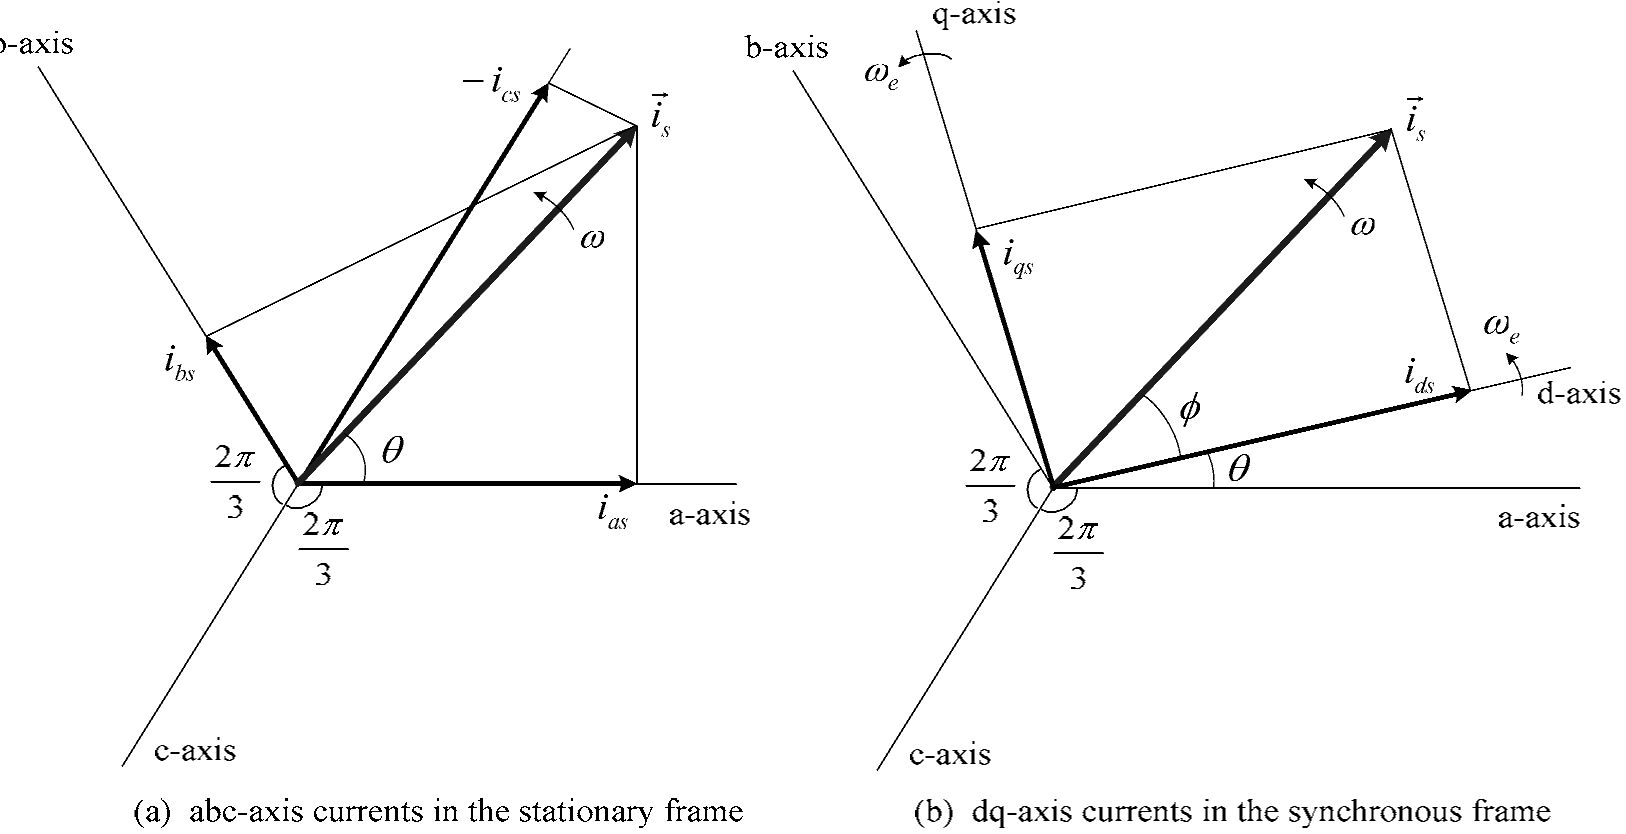
\includegraphics{graficos/img02.jpg}
\caption{Figura 14.2-2: Descomposición del vector de corriente $\vec{i}_s$.}
\end{figure}
\FloatBarrier

La Figura 14.2-2b ilustra otro caso donde el vector de corriente $\vec{i}_s$ está en el marco de referencia síncrono de ejes dq. Suponiendo que $\vec{i}_s$ rota a la misma velocidad que la del marco de referencia de ejes dq, el ángulo de corriente del estator $\phi$, que es el ángulo entre $\vec{i}_s$ y el eje d, es constante. Los componentes resultantes de corriente de los ejes dq, $i_{ds}$ e $i_{qs}$, son señales de corriente continua (dc). Como se verá en las secciones siguientes, esta transformación puede ser utilizada para simplificar la simulación, el diseño y la implementación digital de sistemas de drives, donde una señal de corriente alterna trifásica puede ser representada efectivamente por una señal de corriente continua bifásica.

\subsection{Transformación Estacionaria 3/2}

Con la velocidad de rotación del marco de referencia bifásico fijada en cero y su eje d coincidiendo con el eje a del marco trifásico ($\omega_e = 0$ y $\theta = 0$), ambos marcos son estacionarios en el espacio. La transformación de las variables trifásicas a las variables bifásicas se puede obtener fijando $\theta$ en (14.2-1) a cero, de donde

\begin{equation}
\begin{bmatrix}
x_d \\
x_q
\end{bmatrix}
=
\frac{2}{3}
\begin{bmatrix}
1 & -1/2 & -1/2 \\
0 & \sqrt{3}/2 & -\sqrt{3}/2
\end{bmatrix}
\begin{bmatrix}
x_a \\
x_b \\
x_c
\end{bmatrix} \tag{14.2-6}
\end{equation}

La transformación anterior se denomina transformación 3/2 en este libro. Vale la pena señalar que la variable del eje d se puede expresar como

\begin{equation}
x_d = \frac{2}{3} \left( x_a - \frac{1}{2}x_b - \frac{1}{2}x_c \right) = x_a \tag{14.2-7}
\end{equation}

que es igual a la variable del eje a $x_a$.

De manera similar, la transformación de variables bifásicas a trifásicas estacionarias, que se denota como transformación 2/3, se puede realizar mediante

\begin{equation}
\begin{bmatrix}
x_a \\
x_b \\
x_c
\end{bmatrix}
=
\begin{bmatrix}
1 & 0 \\
-1/2 & \sqrt{3}/2 \\
-1/2 & -\sqrt{3}/2
\end{bmatrix}
\begin{bmatrix}
x_d \\
x_q
\end{bmatrix} \tag{14.2-8}
\end{equation}

\section{Modelos Dinámicos del Motor de Inducción}

Existen dos modelos dinámicos comúnmente utilizados para el motor de inducción. Uno se basa en la teoría del vector espacial y el otro se deriva de la teoría del eje dq. El modelo de vector espacial presenta expresiones matemáticas compactas y un diagrama conciso de vector espacial, mientras que el modelo del eje dq no necesita usar números o variables complejas. Ambos modelos son igualmente válidos para el análisis del rendimiento transitorio y en estado estacionario del motor de inducción. A continuación, se presentan los dos modelos y se revela su relación.

\clearpage
\subsection{Modelo del Motor con Vector Espacial}

En el siguiente análisis se asume que el motor de inducción es trifásico y simétrico, y que su núcleo magnético es lineal con una pérdida de núcleo despreciable. El modelo de vector espacial para un motor de inducción generalmente se compone de tres conjuntos de ecuaciones [2]. El primer conjunto son las ecuaciones de voltaje, dadas por

\begin{equation}
\vec{v}_s = R_s \vec{i}_s + p \vec{\lambda}_s + j\omega \vec{\lambda}_s \tag{14.3-1}
\end{equation}

\begin{equation}
\vec{v}_r = R_r \vec{i}_r + p \vec{\lambda}_r + j(\omega - \omega_r)\vec{\lambda}_r \tag{14.3-1}
\end{equation}

donde $\vec{v}_s$ y $\vec{v}_r$ son los vectores de voltaje del estator y del rotor, respectivamente; $\vec{i}_s$ y $\vec{i}_r$ son los vectores de corriente del estator y del rotor, respectivamente; $\vec{\lambda}_s$ y $\vec{\lambda}_r$ son los vectores de enlace de flujo del estator y del rotor, respectivamente; $R_s$ y $R_r$ son las resistencias del bobinado del estator y del rotor, respectivamente; $\omega$ es la velocidad de rotación de un marco de referencia arbitrario; $\omega_r$ es la velocidad angular del rotor (eléctrica); y $p$ es el operador derivada ($p = d/dt$).

Los términos $j\omega \vec{\lambda}_s$ y $j(\omega - \omega_r)\vec{\lambda}_r$ en el lado derecho de (14.3-1) se refieren a los voltajes de velocidad, que son inducidos por la rotación del marco de referencia.

El segundo conjunto son las ecuaciones de enlace de flujo

\begin{equation}
\vec{\lambda}_s = L_s \vec{i}_s + L_m \vec{i}_r \tag{14.3-2}
\end{equation}

\begin{equation}
\vec{\lambda}_r = L_r \vec{i}_r + L_m \vec{i}_s \tag{14.3-2}
\end{equation}

donde $L_s = L_{ls} + L_m$ representa la autoinductancia del estator; $L_r = L_{lr} + L_m$ representa la autoinductancia del rotor; $L_{ls}$ y $L_{lr}$ son las inductancias de fuga del estator y del rotor, respectivamente; y $L_m$ es la inductancia de magnetización. Cabe señalar que todos los parámetros y variables del rotor, como $R_r$, $L_{lr}$, $\vec{i}_r$ y $\vec{\lambda}_r$, en las ecuaciones anteriores se refieren al lado del estator.

El tercer conjunto es la ecuación de movimiento, dada por

\begin{equation}
\frac{J}{P} p\omega_r = T_e - T_L \tag{14.3-3}
\end{equation}

\begin{equation}
T_e = \frac{3P}{2} \text{Re}(\vec{J} \vec{\lambda}_s \vec{i}_s^*) = -\frac{3P}{2} \text{Re}(\vec{J} \vec{\lambda}_r \vec{i}_r^*) \tag{14.3-3}
\end{equation}

donde $J$ es el momento de inercia total del rotor y la carga, $P$ es el número de pares de polos, $T_L$ es el par de carga y $T_e$ es el par electromagnético.

Las ecuaciones anteriores constituyen el modelo de vector espacial del motor de inducción cuya representación esquemática se muestra en la Fig. 14.3-1. El modelo del motor está en el marco de referencia arbitrario que rota en el espacio a la velocidad arbitraria de $\omega$.

\begin{figure}[ht]
\centering
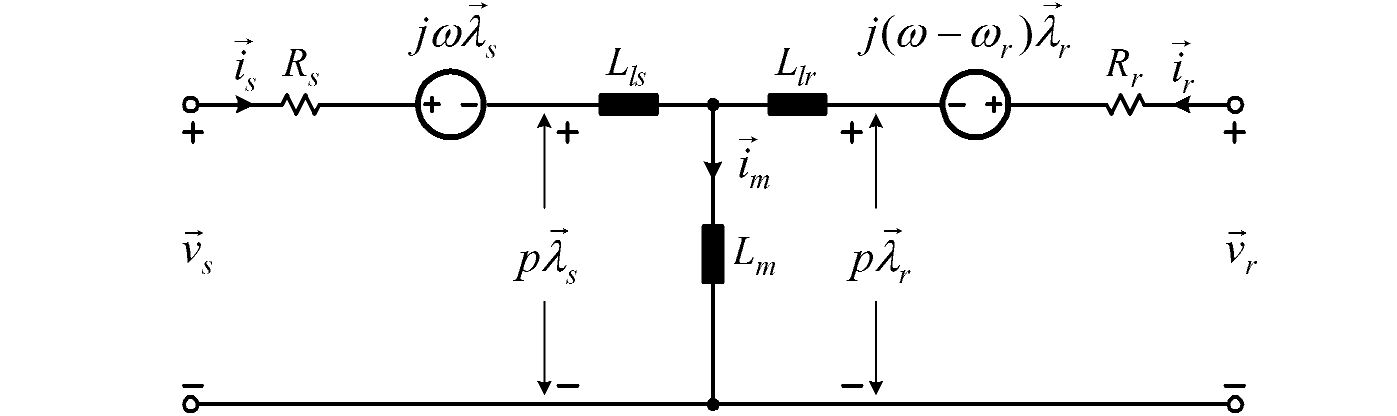
\includegraphics{graficos/img03.jpg}
\caption{Figura 14.3-1: Modelo de vector espacial de un motor de inducción en el marco de referencia arbitrario.}
\end{figure}
\FloatBarrier

En la simulación e implementación digital de sistemas de control avanzados, a menudo se utilizan los modelos de motor en los marcos de referencia síncrono y estacionario. El modelo de motor en el marco síncrono se puede obtener fácilmente fijando la velocidad arbitraria $\omega$ en (14.3-1) a la velocidad síncrona $\omega_e$. La Figura 14.3-2a muestra el circuito equivalente de un motor de jaula de ardilla en el marco síncrono, donde el bobinado del rotor está en cortocircuito ($\vec{v}_r = 0$) y $\omega_{sl}$ es la frecuencia de deslizamiento angular, dada por

\begin{equation}
\omega_{sl} = \omega_e - \omega_r \tag{14.3-4}
\end{equation}

Para obtener el modelo en el marco estacionario (estator), podemos fijar la velocidad arbitraria $\omega$ del marco de referencia rotatorio a cero. El circuito equivalente resultante se muestra en la Fig. 14.3-2b.

\begin{figure}[ht]
\centering
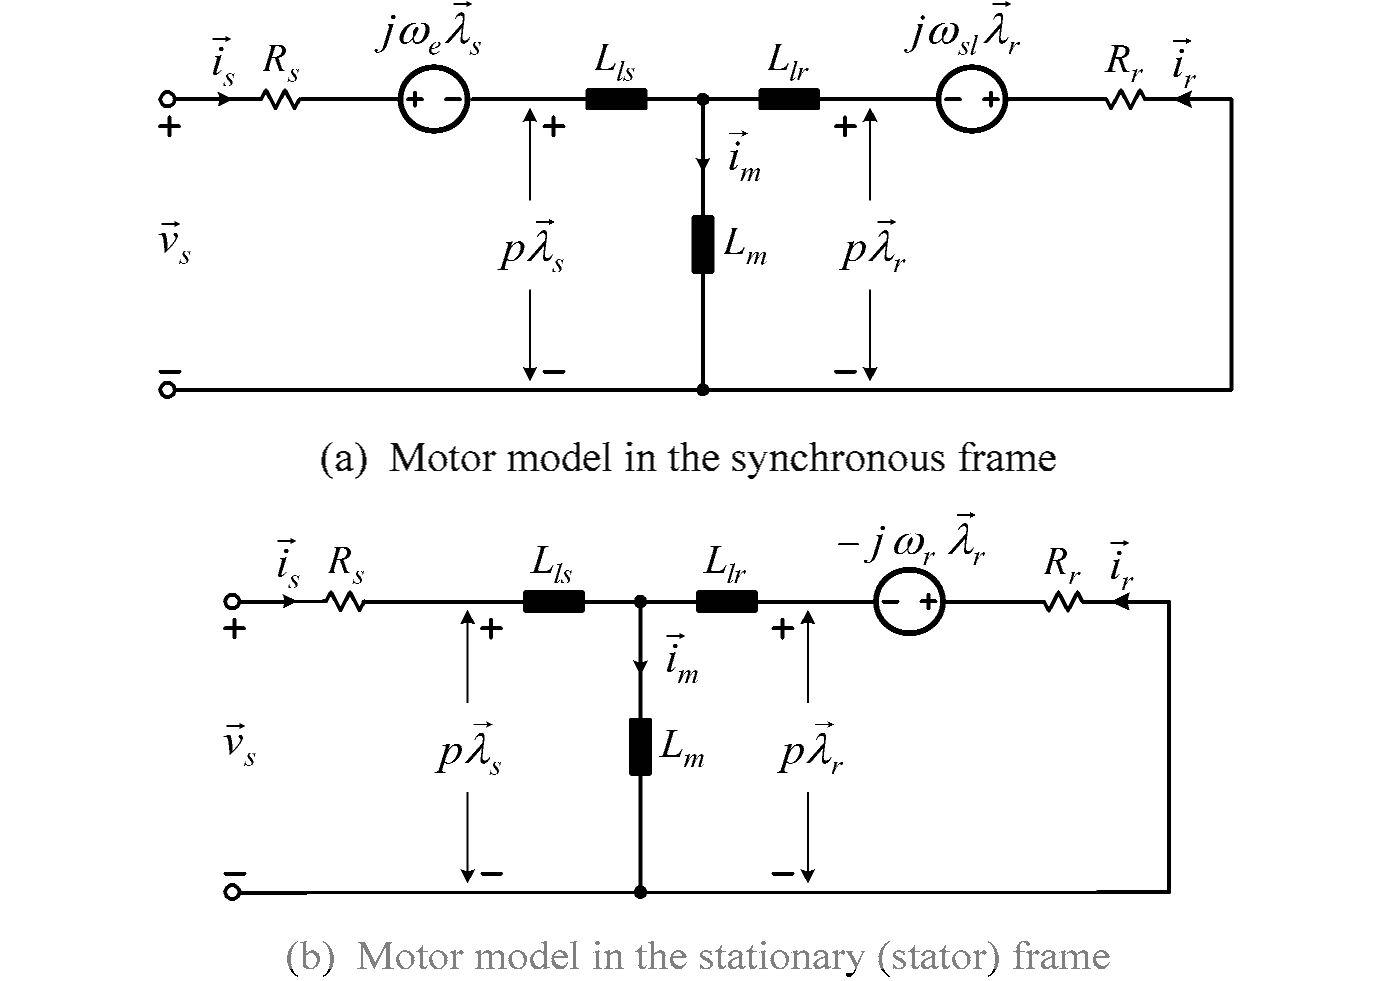
\includegraphics{graficos/img04.jpg}
\caption{Figura 14.3-2: Modelos de vector espacial para un motor de inducción de jaula de ardilla.}
\end{figure}
\FloatBarrier

\subsection{Modelo del Motor en el Eje dq}

El modelo del motor de inducción en el eje dq se puede derivar utilizando la teoría de circuitos trifásicos y luego transformarse al marco bifásico (eje dq) [1]. Alternativamente, también se puede obtener descomponiendo los vectores espaciales en el modelo de motor de vector espacial en los componentes del eje d y q [2], es decir,

\begin{equation}
\vec{v}_s = v_{ds} + jv_{qs}, \quad \vec{i}_s = i_{ds} + ji_{qs}, \quad \vec{\lambda}_s = \lambda_{ds} + j\lambda_{qs} \tag{14.3-5}
\end{equation}

\begin{equation}
\vec{v}_r = v_{dr} + jv_{qr}, \quad \vec{i}_r = i_{dr} + ji_{qr}, \quad \vec{\lambda}_r = \lambda_{dr} + j\lambda_{qr} \tag{14.3-5}
\end{equation}

Sustituyendo (14.3-5) en (14.3-1), se pueden obtener las ecuaciones de voltaje del eje dq para el motor de inducción:

\begin{equation}
v_{ds} = R_s i_{ds} + p\lambda_{ds} - \omega \lambda_{qs} \tag{14.3-6}
\end{equation}
\begin{equation}
v_{qs} = R_s i_{qs} + p\lambda_{qs} + \omega \lambda_{ds} \tag{14.3-6}
\end{equation}
\begin{equation}
v_{dr} = R_r i_{dr} + p\lambda_{dr} - (\omega - \omega_r)\lambda_{dr} \tag{14.3-6}
\end{equation}
\begin{equation}
v_{qr} = R_r i_{qr} + p\lambda_{qr} + (\omega - \omega_r)\lambda_{dr} \tag{14.3-6}
\end{equation}

donde los enlaces de flujo del estator y del rotor se pueden calcular por

\begin{equation}
\lambda_{ds} = L_s i_{ds} + L_m (i_{ds} + i_{dr}) \tag{14.3-7}
\end{equation}
\begin{equation}
\lambda_{qs} = L_s i_{qs} + L_m (i_{qs} + i_{qr}) \tag{14.3-7}
\end{equation}
\begin{equation}
\lambda_{dr} = L_r i_{dr} + L_m (i_{ds} + i_{dr}) \tag{14.3-7}
\end{equation}
\begin{equation}
\lambda_{qr} = L_r i_{qr} + L_m (i_{qs} + i_{qr}) \tag{14.3-7}
\end{equation}

El par electromagnético se puede expresar de varias formas. Algunas de las expresiones comúnmente utilizadas son

\begin{equation}
T_e = \left\{
\begin{array}{l}
\frac{3P}{2}(i_{qs}\lambda_{ds} - i_{ds}\lambda_{qs}) \\
\frac{3PL_m}{2}(i_{qs}i_{dr} - i_{ds}i_{qr}) \\
\frac{3PL_m}{2L_r}(i_{qs}\lambda_{dr} - i_{ds}\lambda_{qr})
\end{array} \tag{14.3-8}
\right.
\end{equation}

Las ecuaciones (14.3-6) a (14.3-8) junto con la ecuación de movimiento de (14.3-3) representan el modelo del motor de inducción en el eje dq, cuyo circuito equivalente se muestra en la Fig. 14.3-3.

\begin{figure}[ht]
\centering
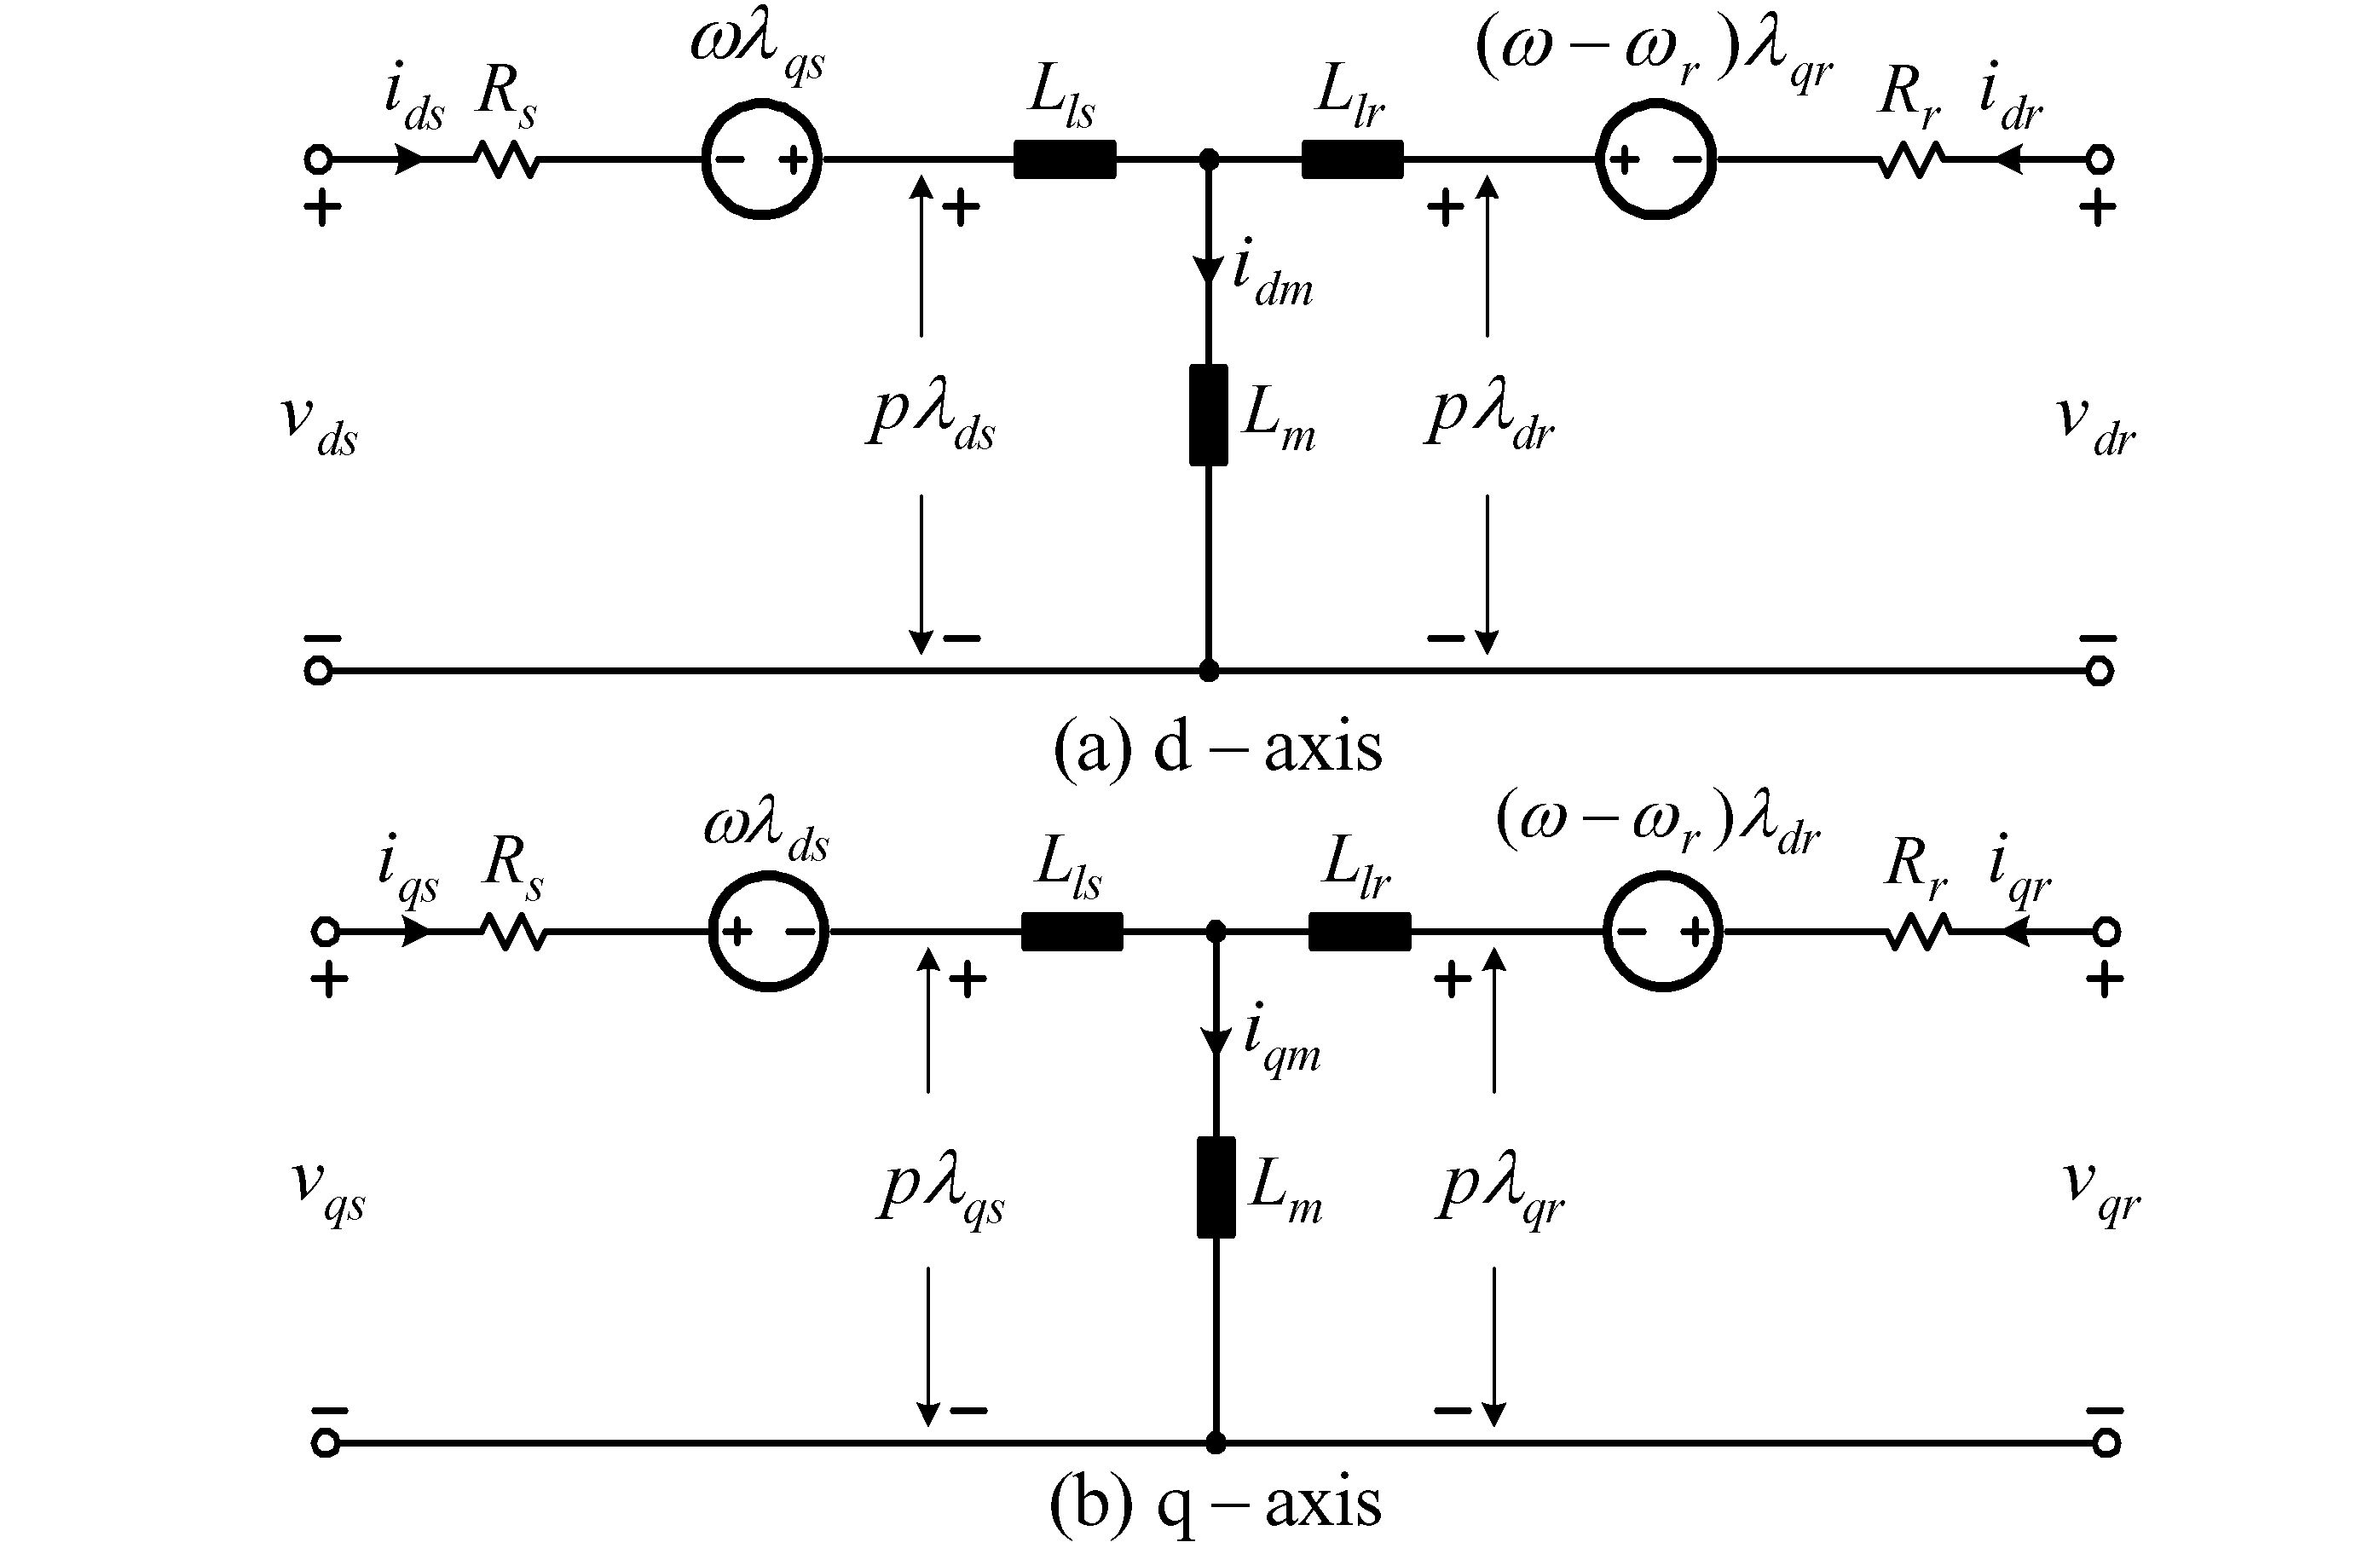
\includegraphics{graficos/img05.jpg}
\caption{Figura 14.3-3: Modelo del motor de inducción en el eje dq en el marco de referencia arbitrario.}
\end{figure}
\FloatBarrier

\subsection{Características Transitorias del Motor de Inducción}

Es instructivo estudiar las características transitorias del motor de inducción durante la aceleración libre utilizando los modelos dinámicos del motor. El motor bajo investigación es un motor de jaula de ardilla de baja potencia con los siguientes parámetros: $V_{LL} = 208 \, V$, 60Hz, $Z_{base} = 15.4 \, \Omega$, $R_s = 0.068 \, pu$, $R_r = 0.045 \, pu$, $L_{ls} = L_{lr} = 0.058 \, pu$, $L_m = 1.95 \, pu$, $P = 1$ y $J = 0.02 \, kg\cdot m^2$. La Figura 14.3-4 muestra el diagrama de bloques para la simulación por computadora con el modelo del motor en el marco estacionario ($\omega = 0$). Los voltajes de suministro trifásico $v_{as}$, $v_{bs}$ y $v_{cs}$ se transforman a los voltajes del estator en el eje dq $v_{ds}$ y $v_{qs}$ mediante la transformación 3/2. Las corrientes simuladas del estator en el eje dq $i_{ds}$ e $i_{qs}$ se convierten luego en las corrientes trifásicas $i_{as}$, $i_{bs}$ e $i_{cs}$ mediante la transformación 2/3.

\begin{figure}[ht]
\centering
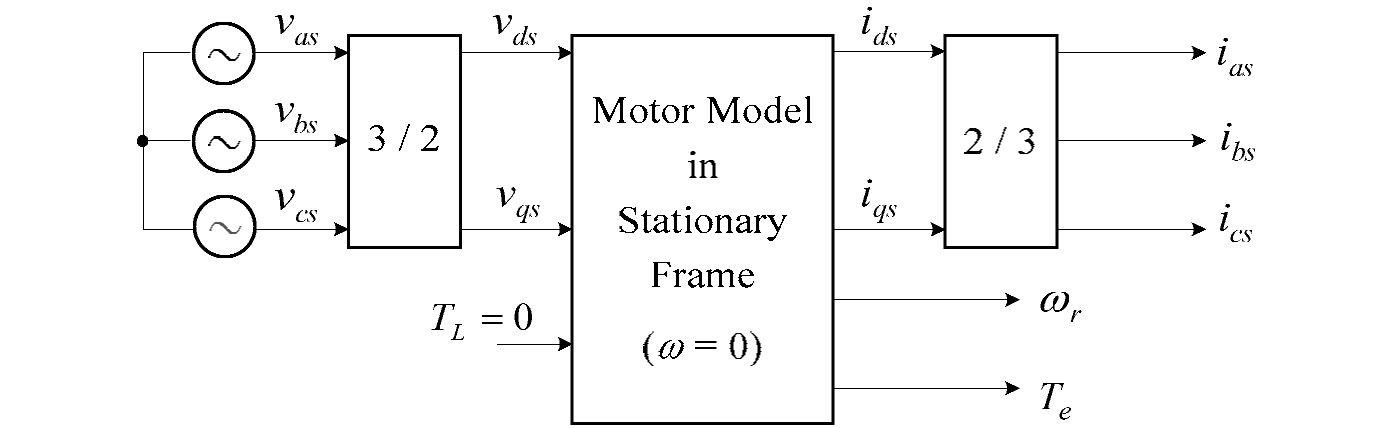
\includegraphics{graficos/img06.jpg}
\caption{Figura 14.3-4: Diagrama de bloques para la simulación de la aceleración libre del motor utilizando el modelo del motor en el marco estacionario.}
\end{figure}
\FloatBarrier

\begin{figure}[ht]
\centering
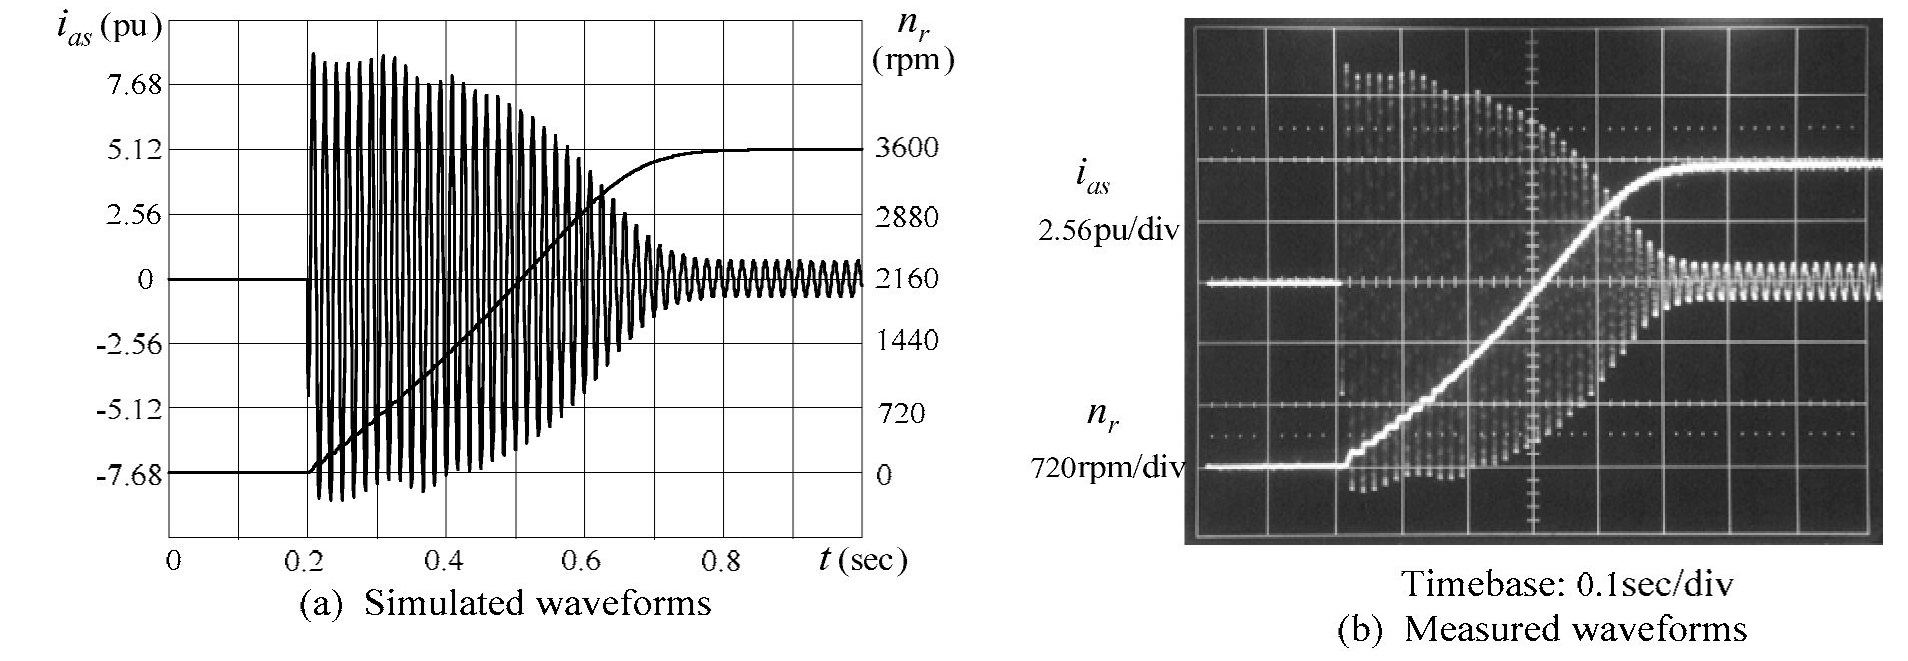
\includegraphics{graficos/img07.jpg}
\caption{Figura 14.3-5: Formas de onda de un motor de inducción durante la aceleración libre.}
\end{figure}
\FloatBarrier

La Figura 14.3-5a muestra las formas de onda transitorias simuladas de la corriente del estator $i_{as}$ y la velocidad del rotor $n_r$ durante la aceleración libre del motor (el motor arranca bajo el voltaje y frecuencia nominales sin carga mecánica). La velocidad del rotor $n_r$, en rpm se relaciona con la velocidad angular eléctrica del rotor $\omega_r$ mediante

\begin{equation}
n_r = \frac{30}{\pi P} \omega_r \tag{14.3-9}
\end{equation}

La corriente de arranque pico es aproximadamente 8.4 pu, lo que representa una corriente de arranque rms de 5.9 pu. El tiempo de arranque es de alrededor de 0.5 s debido al bajo momento de inercia y alta corriente de arranque. Las formas de onda medidas durante la aceleración libre se muestran en la Fig. 14.3-5b, que coinciden muy bien con los resultados simulados.

\begin{figure}[ht]
\centering
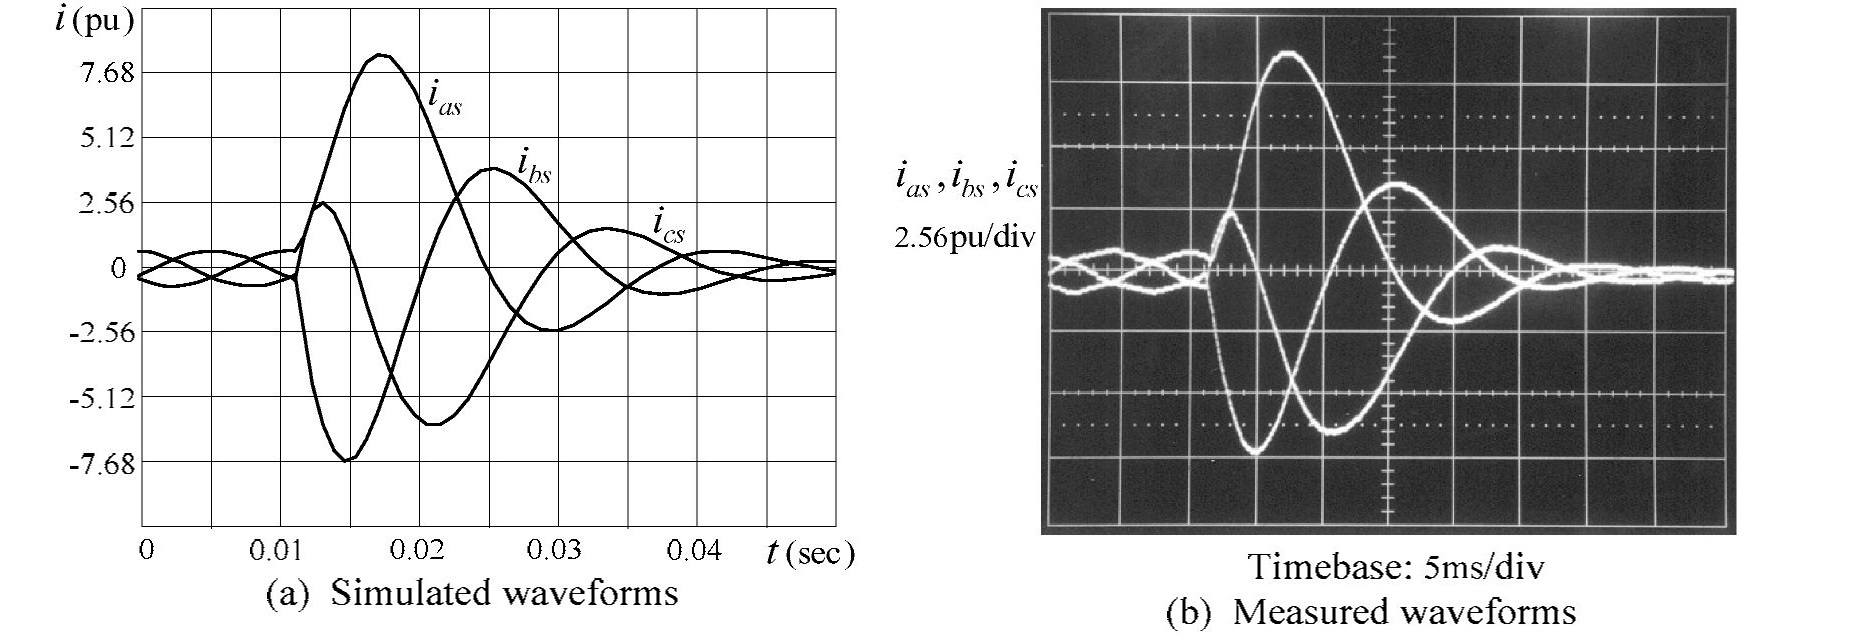
\includegraphics{graficos/img08.jpg}
\caption{Figura 14.3-6: Formas de onda de la corriente del estator de un motor de inducción durante una falla trifásica.}
\end{figure}
\FloatBarrier

La Figura 14.3-6 muestra las formas de onda transitorias simuladas y medidas del motor durante una falla trifásica. El motor opera cerca de su velocidad síncrona cuando sus terminales trifásicos están en cortocircuito. La corriente pico máxima del estator es cercana a la durante la aceleración libre. Las formas de onda medidas se correlacionan estrechamente con las simuladas.

\begin{figure}[ht]
\centering
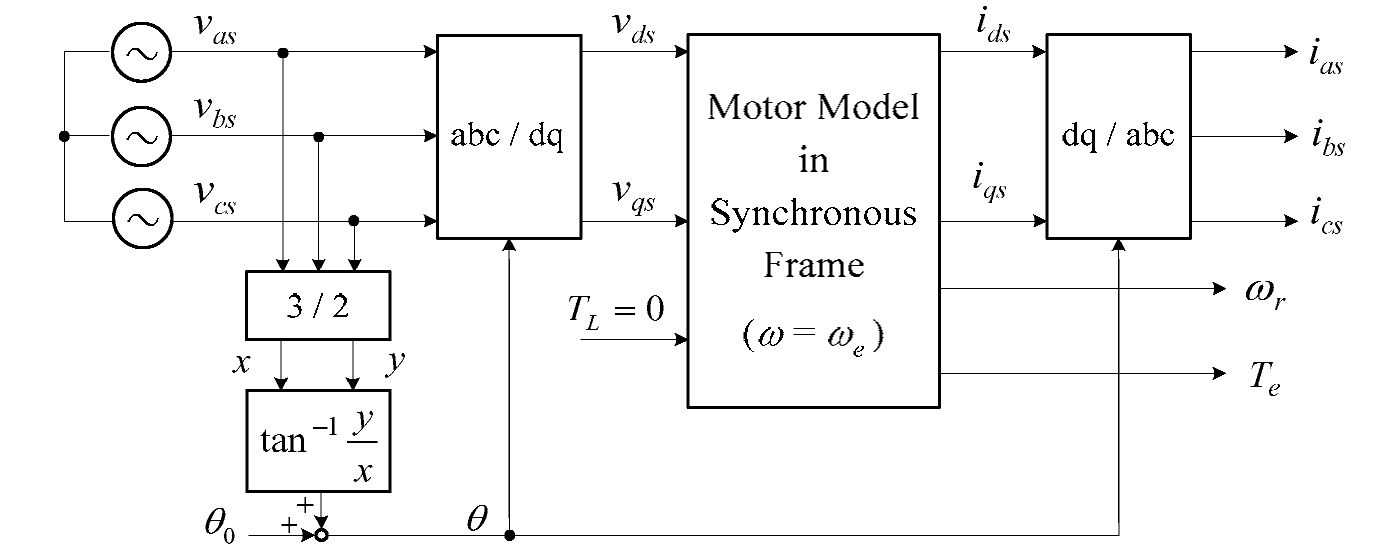
\includegraphics{graficos/img09.jpg}
\caption{Figura 14.3-7: Diagrama de bloques para la simulación de la aceleración libre del motor utilizando el modelo del motor en el marco síncrono.}
\end{figure}
\FloatBarrier

La Figura 14.3-7 ilustra el diagrama de bloques de simulación con el modelo del motor en el marco síncrono. Utilizando los bloques de transformación abc/dq y dq/abc, los voltajes de suministro trifásico $v_{as}$, $v_{bs}$ y $v_{cs}$ en el marco estacionario se pueden transformar a los voltajes del eje dq $v_{ds}$ y $v_{qs}$ en el marco síncrono, mientras que las corrientes simuladas del eje dq $i_{ds}$ e $i_{qs}$ en el marco síncrono se pueden convertir en corrientes trifásicas $i_{as}$, $i_{bs}$ y $i_{cs}$ en el marco estacionario. El ángulo $\theta$ en los bloques de transformación se puede obtener mediante la transformación 3/2 y los bloques tan$^{-1}$ mostrados en la figura o utilizando directamente la Ec. (14.2-3).

\begin{figure}[ht]
\centering
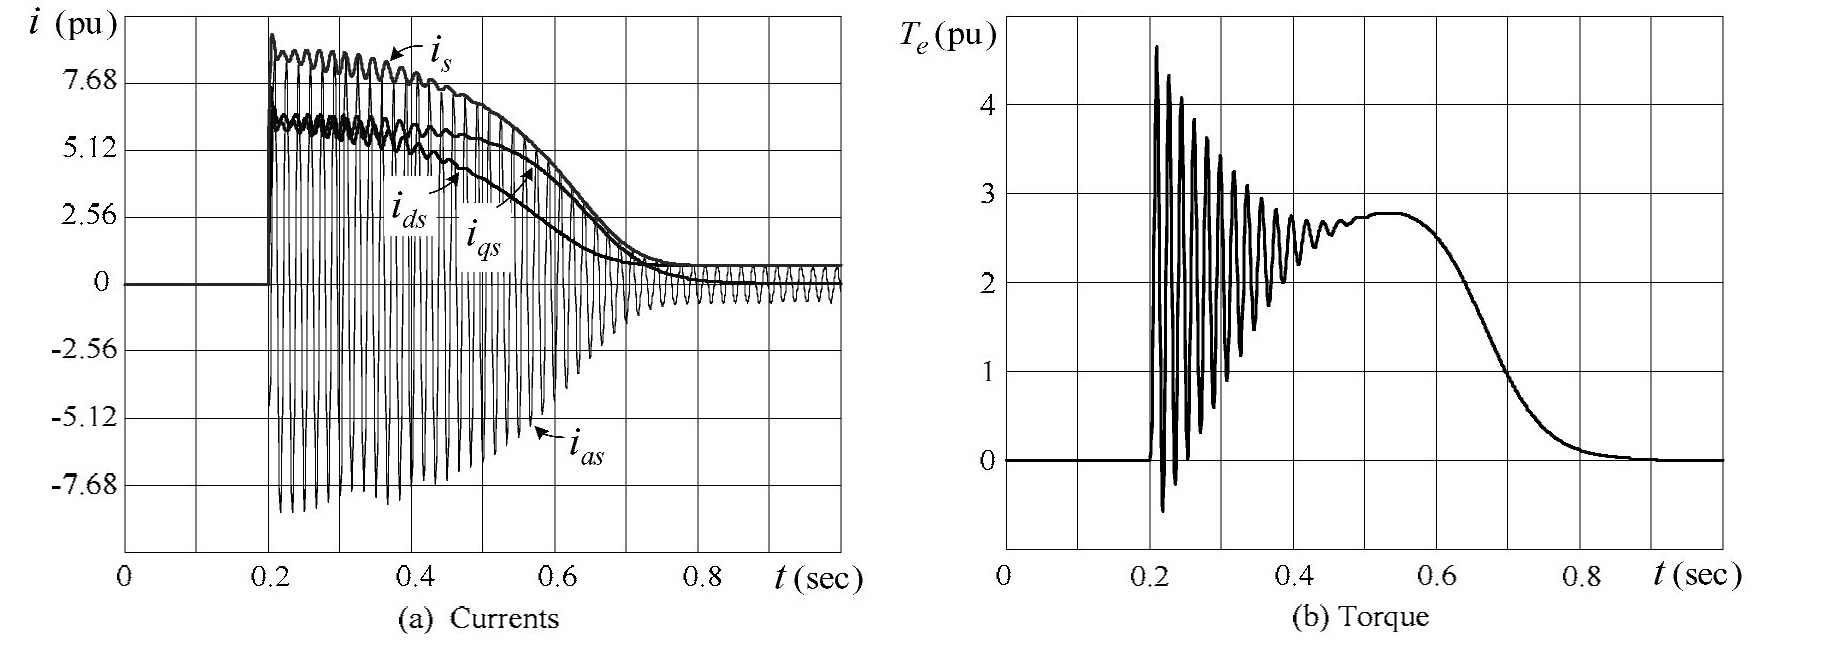
\includegraphics{graficos/img10.jpg}
\caption{Figura 14.3-8: Formas de onda simuladas para la aceleración libre del motor utilizando el modelo del motor en el marco síncrono.}
\end{figure}
\FloatBarrier

La Figura 14.3-8a muestra las formas de onda simuladas para $i_{as}$, $i_{ds}$ y $i_{qs}$ durante la aceleración libre del motor. La forma de onda de $i_{as}$ en el marco estacionario es exactamente la misma que la de la Fig. 14.3-5. Las corrientes del eje dq $i_{ds}$ e $i_{qs}$ están en el marco síncrono y, por lo tanto, son señales de corriente continua (dc) en estado estacionario. La amplitud de la corriente del estator $\vec{i}_s$ se puede obtener mediante $\vec{i}_s = \sqrt{i_{ds}^2 + i_{qs}^2}$. Los voltajes del eje dq $v_{ds}$ y $v_{qs}$ en el marco síncrono son constantes de corriente continua y, por lo tanto, no se muestran en la figura.

El ángulo de corriente del estator $\phi$, que es el ángulo entre $\vec{i}_s$ y el eje d como se muestra en la Fig. 14.2-2b, afectará las formas de onda de $i_{ds}$ e $i_{qs}$. Las formas de onda en la Fig. 14.3-8a se obtienen con $\phi = 0$ ajustando el ángulo inicial $\theta_0$ de modo que el eje d del marco síncrono esté alineado con $\vec{i}_s$. Esto lleva a $i_{qs} = 0$ y $i_{ds} = i_s$ cuando el motor está en operación en estado estacionario. Si el eje q del marco síncrono está alineado con $\vec{i}_s$ ($\phi = 90^\circ$), las corrientes del eje dq en estado estacionario son $i_{qs} = i_s$ y $i_{ds} = 0$. Sin embargo, la forma de onda de $i_s$ no se ve afectada por $\phi$.

La respuesta del par durante la aceleración libre del motor se muestra en la Fig. 14.3-8b. Aunque se obtiene con el modelo del motor en el marco síncrono, la respuesta sigue siendo la misma para el modelo del motor en cualquier otro marco de referencia.

\section{Principio del Control Orientado al Campo (FOC)}

\subsection{Orientación del Campo}

Es bien sabido que el drive de motor de corriente continua (dc) tiene un excelente rendimiento dinámico. Esto se debe principalmente al control desacoplado (separado) del campo magnético del estator y el par electromagnético del motor. El par se desarrolla por la interacción de dos campos magnéticos perpendiculares. Un campo es generado por la corriente de campo $i_f$ en el bobinado del estator, y el otro es producido por la corriente del inducido (rotor) $i_a$. El par desarrollado se puede expresar como

\begin{equation}
T_e = K_a \lambda_f i_a \tag{14.4-1}
\end{equation}

donde $K_a$ es una constante del inducido y $\lambda_f$ es el flujo producido por $i_f$. En los drives de dc de alto rendimiento, $\lambda_f$ normalmente se mantiene constante manteniendo $i_f$ constante, y así el par $T_e$ es proporcional a y puede ser controlado directamente por $i_a$.

El control orientado al campo, también conocido como control vectorial, para el motor de inducción emula el control del motor de dc. Usando una orientación de campo adecuada, la corriente del estator puede descomponerse en un componente que produce flujo y un componente que produce par. Estos dos componentes se controlan por separado.

La orientación del campo se puede clasificar generalmente en orientaciones de flujo del estator, flujo del entrehierro y flujo del rotor [3, 4]. Dado que la orientación del flujo del rotor se utiliza ampliamente en los drives de corriente alterna (ac), se analizará este esquema en detalle. Su principio de funcionamiento se puede aplicar fácilmente a los otros dos esquemas de orientación del campo.

\begin{figure}[ht]
\centering
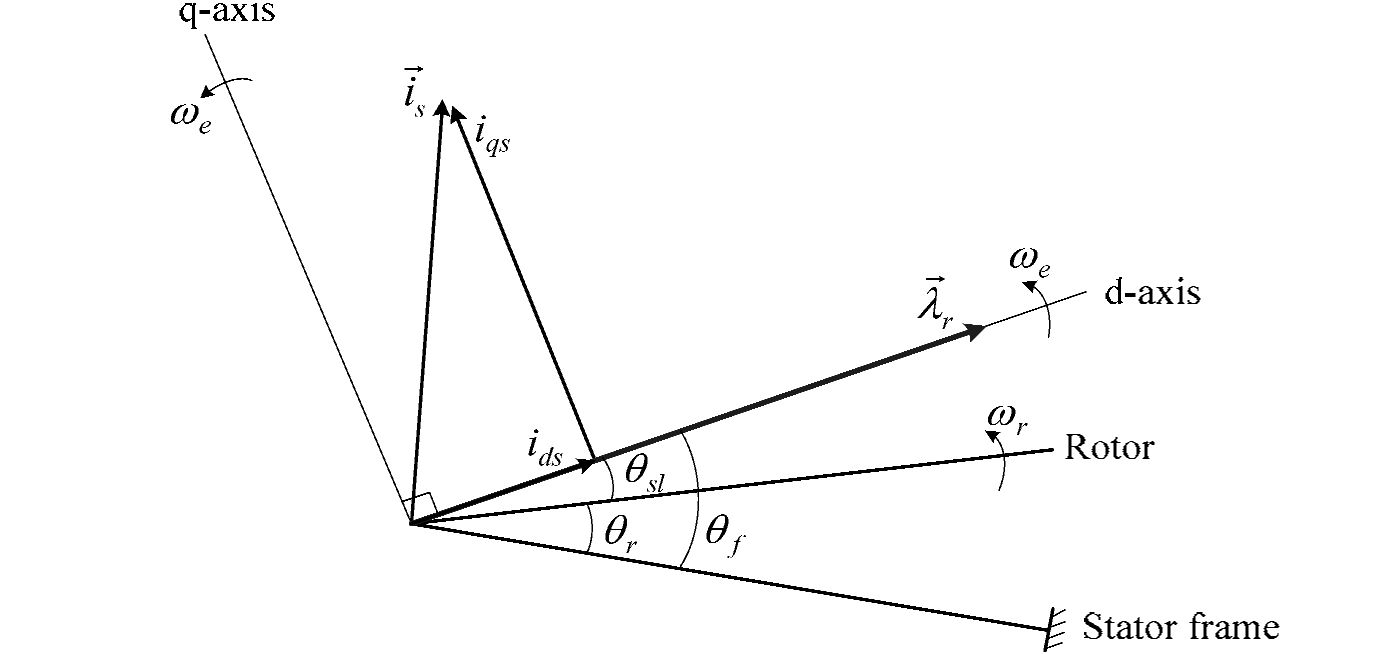
\includegraphics{graficos/img11.jpg}
\caption{Figura 14.4-1: Orientación del campo de flujo del rotor (el eje d está alineado con $\vec{\lambda}_r$).}
\end{figure}
\FloatBarrier

La orientación del flujo del rotor se logra alineando el eje d del marco de referencia síncrono con el vector de flujo del rotor $\vec{\lambda}_r$ como se muestra en la Fig. 14.4-1. Los componentes de flujo del rotor en los ejes d y q resultantes son

\begin{equation}
\lambda_{qr} = 0 \quad \text{y} \quad \lambda_{dr} = \lambda_r \tag{14.4-2}
\end{equation}

donde $\lambda_r$ es la magnitud de $\vec{\lambda}_r$. Sustituyendo (14.4-2) en la última ecuación de (14.3-8) se obtiene

\begin{equation}
T_e = K_r \lambda_r i_{qs} = K_r \lambda_r i_{qs} \tag{14.4-3}
\end{equation}

donde $K_r = 3PL_m/2L_r$. La ecuación (14.4-3) indica que con la orientación del campo del rotor la expresión del par para el motor de inducción es similar a la de un motor de dc. Si $\lambda_r$ puede mantenerse constante durante el funcionamiento del motor, el par desarrollado puede ser controlado directamente por la corriente del estator en el eje q $i_{qs}$.

El vector de corriente del estator $\vec{i}_s$ en la Fig. 14.4-1 se puede resolver en dos componentes a lo largo de los ejes dq. La corriente del eje d $i_{ds}$ se refiere como corriente de producción de flujo mientras que la corriente del eje q $i_{qs}$, que es perpendicular a $i_{ds}$, es la corriente de producción de par. En el control orientado al campo, $i_{ds}$ normalmente se mantiene en su valor nominal mientras que $i_{qs}$ se controla de manera independiente. Con el control desacoplado para $i_{ds}$ e $i_{qs}$, se puede realizar un drive de alto rendimiento.

Uno de los problemas clave asociados con el control orientado al flujo del rotor es determinar con precisión el ángulo de flujo del rotor $\theta_f$ para la orientación del campo. Se pueden utilizar varios esquemas para encontrar $\theta_f$. Por ejemplo, se puede calcular a partir de los voltajes y corrientes del estator medidos, o se puede encontrar a partir de

\begin{equation}
\theta_f = \theta_r + \theta_{sl} \tag{14.4-4}
\end{equation}

donde $\theta_r$ y $\theta_{sl}$ son el ángulo de posición del rotor medido y el ángulo de deslizamiento calculado, respectivamente.

\subsection{Diagrama de Bloques General del FOC}

Dependiendo de cómo se obtenga el ángulo de flujo del rotor $\theta_f$, los esquemas de control se pueden clasificar en controles orientados al campo directos e indirectos. Si $\theta_f$ se obtiene utilizando dispositivos de detección de flujo incorporados en el motor o utilizando los voltajes y corrientes terminales del motor medidos, el método se denomina control orientado al campo directo. Si el ángulo de flujo del rotor $\theta_f$ se obtiene a partir del ángulo de posición del rotor detectado $\theta_r$ y el ángulo de deslizamiento calculado $\theta_{sl}$ como se muestra en (14.4-4), este esquema se conoce como \textit{control orientado al campo indirecto} [3, 4].

\begin{figure}[ht]
\centering
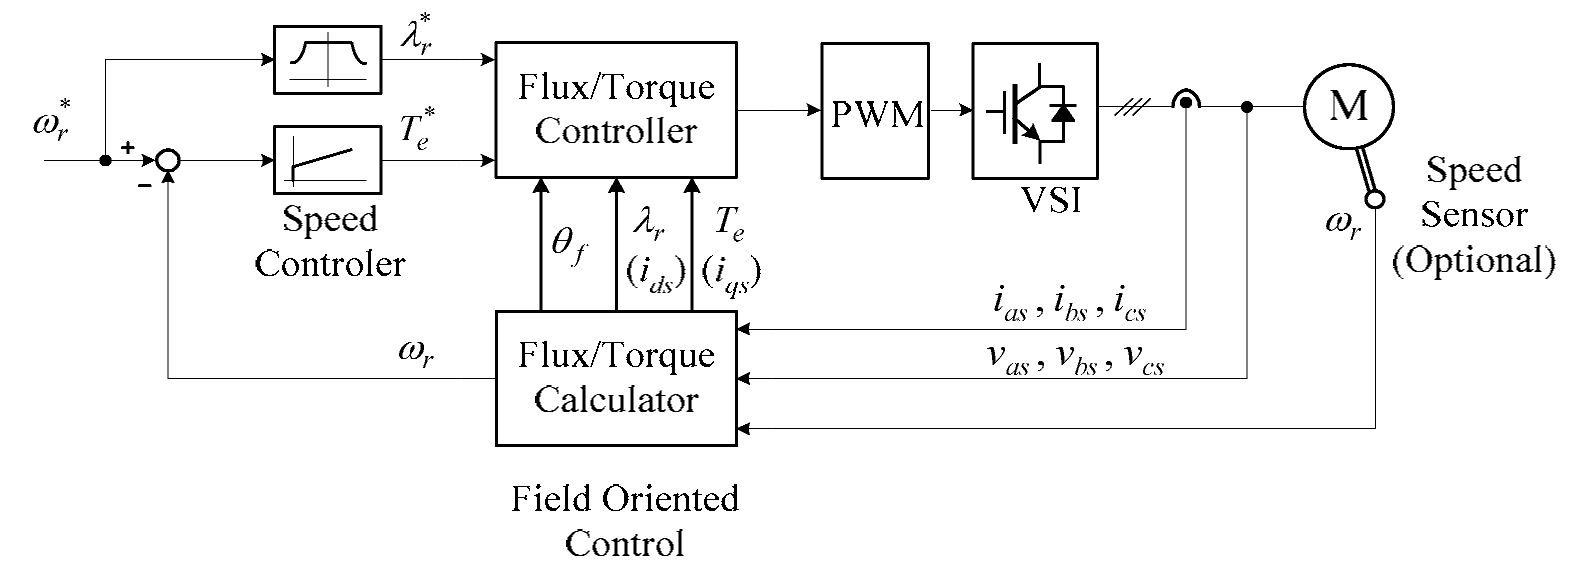
\includegraphics{graficos/img12.jpg}
\caption{Figura 14.4-2: Diagrama de bloques general del FOC orientado al flujo del rotor.}
\end{figure}
\FloatBarrier

Un diagrama de bloques general de un drive de motor de inducción con control orientado al flujo del rotor se muestra en la Fig. 14.4-2. Dado que la esencia del FOC es el control desacoplado del flujo del rotor $\lambda_r$ y el par electromagnético $T_e$, estas dos variables se controlan por separado. La referencia de par $T_e^*$ es generada por el \textit{Controlador de Velocidad} basado en la velocidad de referencia $\omega_r^*$ y la velocidad del rotor detectada o estimada $\omega_r$. La referencia de flujo del rotor $\lambda_r^*$ es una función de $\omega_r^*$. Cuando el motor opera a su velocidad nominal o por debajo de ella, $\lambda_r^*$ normalmente se mantiene en su valor nominal. Con la velocidad nominal excedida, $\lambda_r^*$ debe debilitarse correspondientemente para que el voltaje del estator y la potencia de salida del motor no excedan sus valores nominales.

Las dos referencias $\lambda_r^*$ y $T_e^*$ se envían al \textit{Controlador de Flujo/Par}, donde se comparan con el flujo del rotor calculado $\lambda_r$ y el par $T_e$ para un control en lazo cerrado. El \textit{Controlador de Flujo/Par} genera señales de referencia para el bloque PWM, que produce señales de compuerta para el inversor para ajustar su voltaje y frecuencia de salida.

Basado en las variables de voltaje y corriente del estator medidas y el modelo del motor, el \textit{Calculador de Flujo/Par} calcula (1) el ángulo de flujo del rotor $\theta_f$ para la orientación del campo, (2) la magnitud del flujo del rotor $\lambda_r$ o la corriente de producción de flujo $i_{ds}$, (3) el par electromagnético $T_e$ o la corriente de producción de par $i_{qs}$ y (4) la velocidad del rotor $\omega_r$. Dependiendo de los requisitos del sistema de drive y del tipo de esquema FOC empleado, la velocidad del rotor $\omega_r$ también puede ser detectada directamente por un sensor digital de velocidad. Vale la pena señalar que el \textit{Calculador de Flujo/Par}, también conocido como \textit{Observador de Flujo/Par} o \textit{Estimador} en la literatura, es el bloque funcional más importante en el esquema FOC.

\clearpage
\section{Control Orientado al Campo Directo}

\subsection{Diagrama de Bloques del Sistema}

\begin{figure}[ht]
\centering
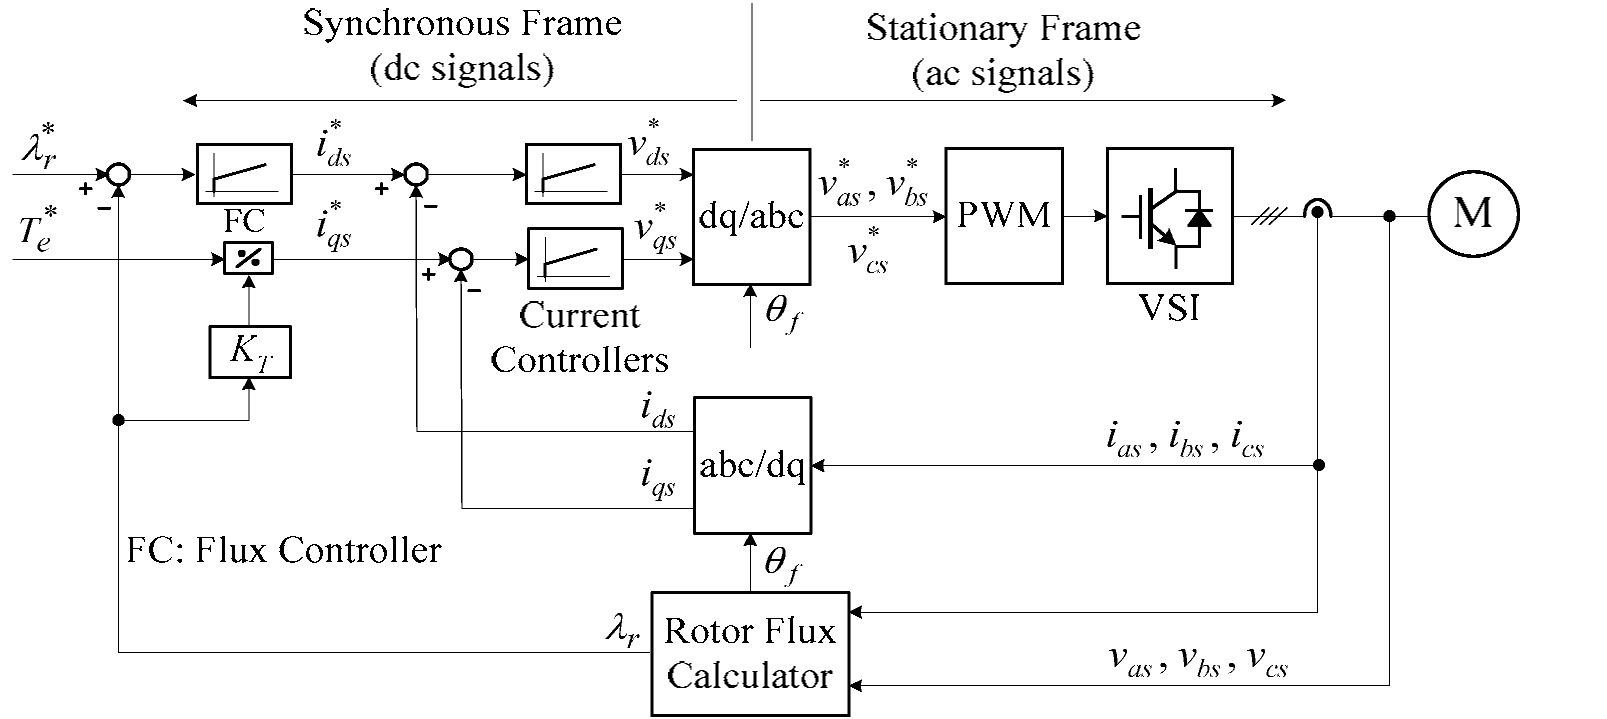
\includegraphics{graficos/img13.jpg}
\caption{Figura 14.5-1: Control orientado al campo directo con orientación al flujo del rotor.}
\end{figure}
\FloatBarrier

La Figura 14.5-1 muestra un diagrama de bloques típico del control orientado al campo directo para el motor de inducción, donde no se muestra el control de velocidad del rotor para mayor simplicidad. Hay tres lazos de control de retroalimentación, uno para el enlace de flujo del rotor $\lambda_r$, uno para la corriente del estator en el eje d (producción de flujo) $i_{ds}$ y otro para la corriente del estator en el eje q (producción de par) $i_{qs}$.

Para el control del flujo del rotor, la $\lambda_r$ calculada se compara con su referencia $\lambda_r^*$ para generar la corriente de referencia del estator en el eje d $i_{ds}^*$ a través del controlador de flujo (FC). La corriente de referencia del estator en el eje q $i_{qs}^*$ se genera según la referencia de par $T_e^*$. Las corrientes de retroalimentación del estator en los ejes dq $i_{ds}$ e $i_{qs}$ se comparan con sus referencias, y los errores se envían a los controladores de corriente para generar las referencias de voltaje del estator $v_{ds}^*$ y $v_{qs}^*$. Los voltajes en el eje dq en el marco síncrono luego se transforman a los voltajes trifásicos del estator $v_{as}^*$, $v_{bs}^*$ y $v_{cs}^*$ en el marco estacionario para el bloque PWM. Se pueden usar varios esquemas de PWM. Si se emplea un esquema de modulación basado en portadora, $v_{as}^*$, $v_{bs}^*$ y $v_{cs}^*$ son las señales de modulación que se comparan con una onda portadora triangular para generar el PWM de compuerta para los dispositivos de conmutación en el inversor.

Como se muestra en la Fig. 14.5-1, el ángulo de flujo del rotor $\theta_f`$ se utiliza en los bloques de transformación abc/dq y dq/abc para la orientación del campo. Las variables a la izquierda de los bloques de transformación son todas señales de corriente continua en el marco síncrono, mientras que las de la derecha de los bloques de transformación son todas variables de corriente alterna en el marco estacionario.

\clearpage
\subsection{Calculador de Flujo del Rotor}

Basado en el modelo del motor en el marco estacionario en la Fig. 14.3-2b, el vector de flujo del estator se puede expresar como

\begin{equation}
\vec{\lambda}_s = \int (\vec{v}_s - R_s \vec{i}_s) \, dt \tag{14.5-1}
\end{equation}

El vector de flujo del rotor se puede encontrar a partir de las ecuaciones de enlace de flujo (14.3-2):

\begin{equation}
\vec{\lambda}_r = L_r \frac{\vec{\lambda}_s - L_s \vec{i}_s}{L_m} + L_m \vec{i}_s = \frac{L_r}{L_m} (\vec{\lambda}_s - \sigma L_s \vec{i}_s) \tag{14.5-2}
\end{equation}

donde $\sigma$ es el factor de fuga total, definido por

\begin{equation}
\sigma = 1 - \frac{L_m^2}{L_s L_r} \tag{14.5-3}
\end{equation}

Descomponiendo el flujo del rotor $\vec{\lambda}_r$ en los componentes de los ejes d y q, tenemos

\begin{equation}
\lambda_{dr} = \frac{L_r}{L_m} (\lambda_{ds} - \sigma L_s i_{ds}) \tag{14.5-4}
\end{equation}
\begin{equation}
\lambda_{qr} = \frac{L_r}{L_m} (\lambda_{qs} - \sigma L_s i_{qs}) \tag{14.5-4}
\end{equation}

a partir de los cuales la magnitud y el ángulo del flujo del rotor son

\begin{equation}
\lambda_r = \sqrt{\lambda_{dr}^2 + \lambda_{qr}^2} \tag{14.5-5}
\end{equation}
\begin{equation}
\theta_r = \tan^{-1} \frac{\lambda_{qr}}{\lambda_{dr}} \tag{14.5-5}
\end{equation}

Se pueden notar las siguientes observaciones de (14.5-1) a (14.5-5):

\begin{itemize}
    \item La magnitud del flujo del rotor $\lambda_r$ y su ángulo $\theta_r$ se pueden identificar basados en el voltaje del estator medido $\vec{v}_s$, la corriente del estator $\vec{i}_s$ y los parámetros del motor ($L_s$, $L_r$, $L_m$ y $R_s$).
    \item Dado que se utiliza el modelo del motor en el marco estacionario, todas las variables como $\lambda_{dr}$, $\lambda_{qr}$, $i_{ds}$ e $i_{qs}$ (excepto $\lambda_r$ y $\theta_r$) son señales de corriente alterna. Descartando los armónicos de conmutación, son sinusoidales en estado estacionario.
\end{itemize}

\begin{figure}[ht]
\centering
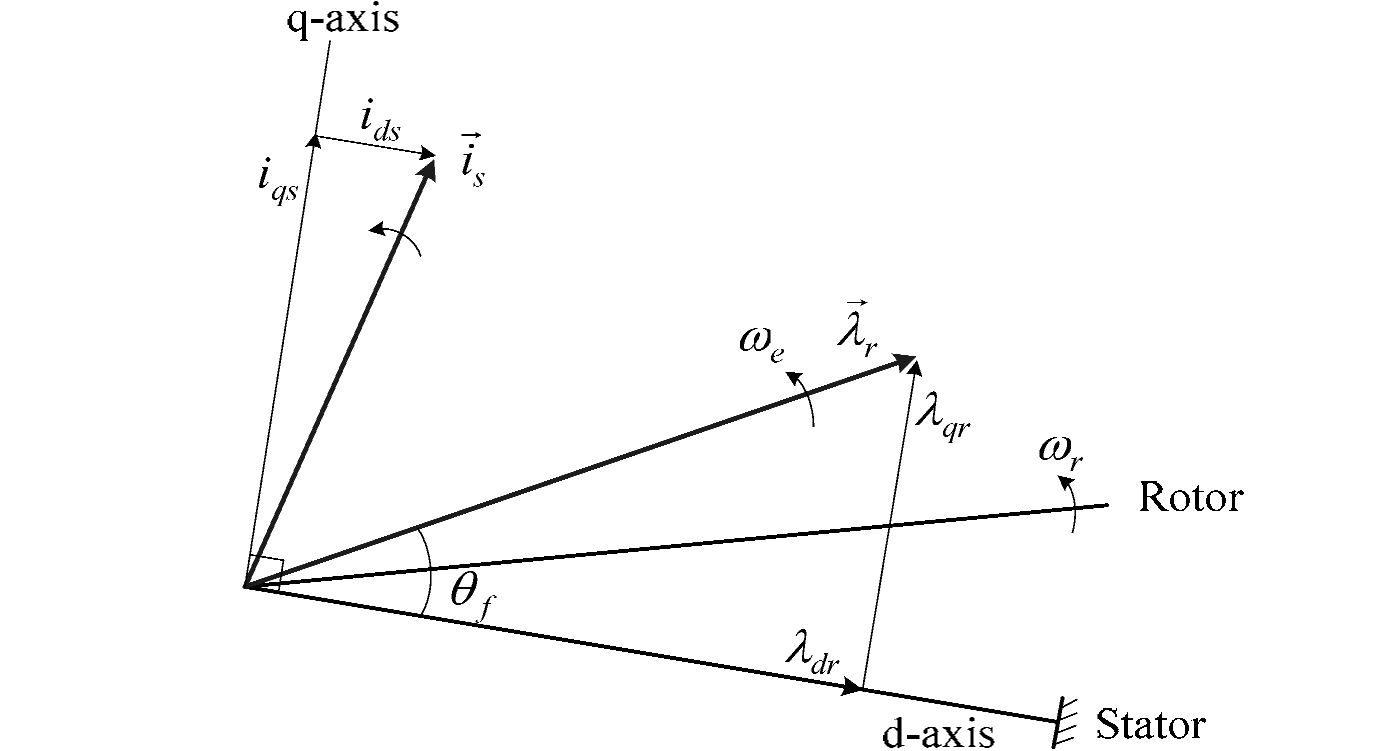
\includegraphics{graficos/img14.jpg}
\caption{Figura 14.5-2: Diagrama vectorial para $\vec{\lambda}_r$ y $\vec{i}_s$ utilizado en el calculador de flujo del rotor.}
\end{figure}
\FloatBarrier

La Figura 14.5-2 muestra el diagrama vectorial para el vector de flujo del rotor $\vec{\lambda}_r$ y el vector de corriente del estator $\vec{i}_s$ utilizado en el Calculador de Flujo del Rotor. Cuando los dos vectores rotan una revolución en el espacio, sus componentes en los ejes dq $\lambda_{dr}$, $\lambda_{qr}$, $i_{ds}$ e $i_{qs}$ en el marco estacionario (estator) varían un ciclo en el tiempo.

\begin{figure}[ht]
\centering
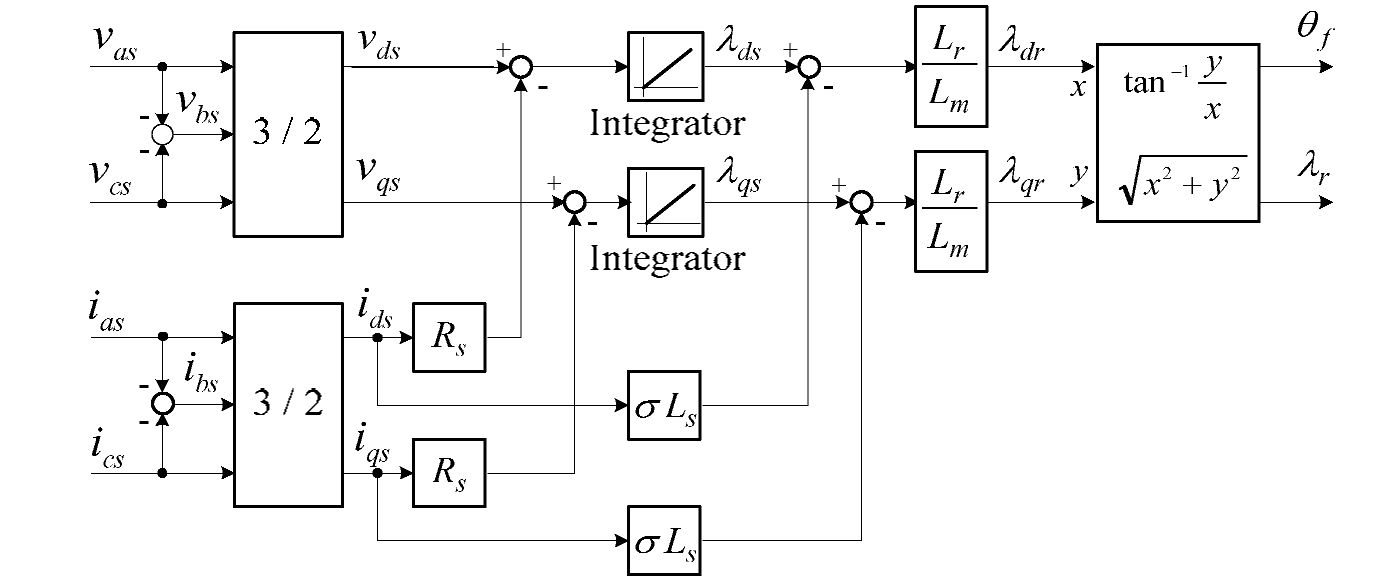
\includegraphics{graficos/img15.jpg}
\caption{Figura 14.5-3: Diagrama de bloques para el cálculo del flujo del rotor.}
\end{figure}
\FloatBarrier

La Figura 14.5-3 muestra el diagrama de bloques para la implementación digital del Calculador de Flujo del Rotor. De los tres voltajes del estator $v_{as}$, $v_{bs}$ y $v_{cs}$, solo se necesitan medir dos y el tercero se puede encontrar a partir de $v_{as} + v_{bs} + v_{cs} = 0$. Para reducir el número de sensores de voltaje, los voltajes del estator también se pueden reconstruir utilizando la función de conmutación del inversor y el voltaje de corriente continua medido. Los voltajes y corrientes del estator se transforman luego a variables bifásicas a través de bloques de transformación estacionaria 3/2. Los otros bloques se derivan de las ecuaciones (14.5-1) a (14.5-5). La salida del Calculador de Flujo del Rotor es el ángulo de flujo del rotor $\theta_f$ y su amplitud $\lambda_r$.

\clearpage
\subsection{FOC Directo con VSI Controlado por Corriente}

\begin{figure}[ht]
\centering
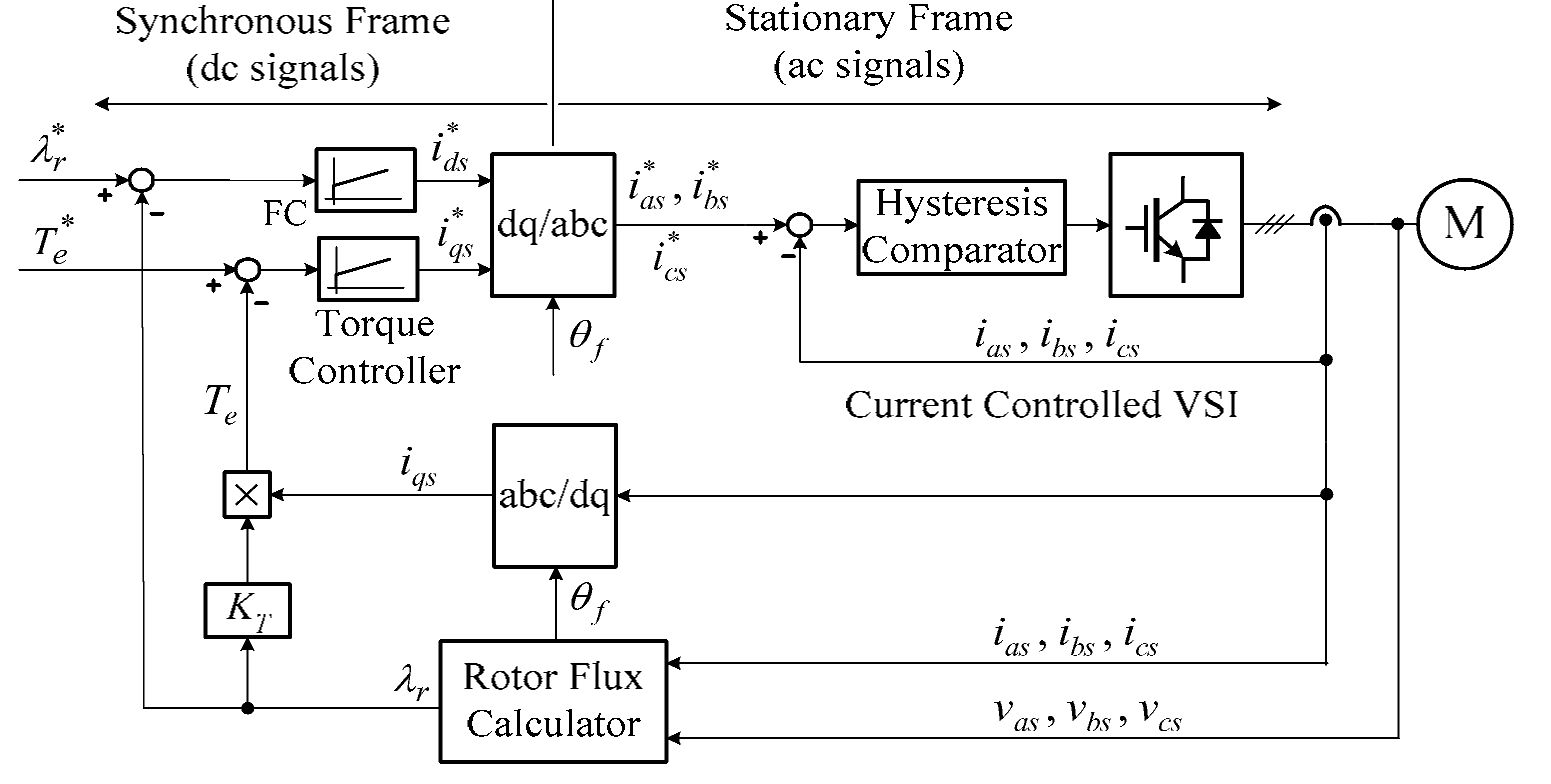
\includegraphics[scale=0.9]{graficos/img16.jpg}
\caption{Figura 14.5-4: FOC directo con un VSI regulado por corriente.}
\end{figure}
\FloatBarrier

El esquema FOC directo discutido en las secciones anteriores se puede simplificar si se utiliza un inversor de fuente de voltaje (VSI) regulado por corriente. La Figura 14.5-4 muestra el diagrama de bloques de un sistema de este tipo. El VSI regulado por corriente puede hacer que las corrientes de salida del inversor $i_{as}$, $i_{bs}$ e $i_{cs}$ sigan sus referencias $i_{as}^*$, $i_{bs}^*$ e $i_{cs}^*$ de cerca. Por lo tanto, no es necesario usar los controladores de corriente en la Fig. 14.5-1. Además, el esquema PWM para el VSI regulado por corriente es más simple que otras técnicas de modulación.

\begin{figure}[ht]
\centering
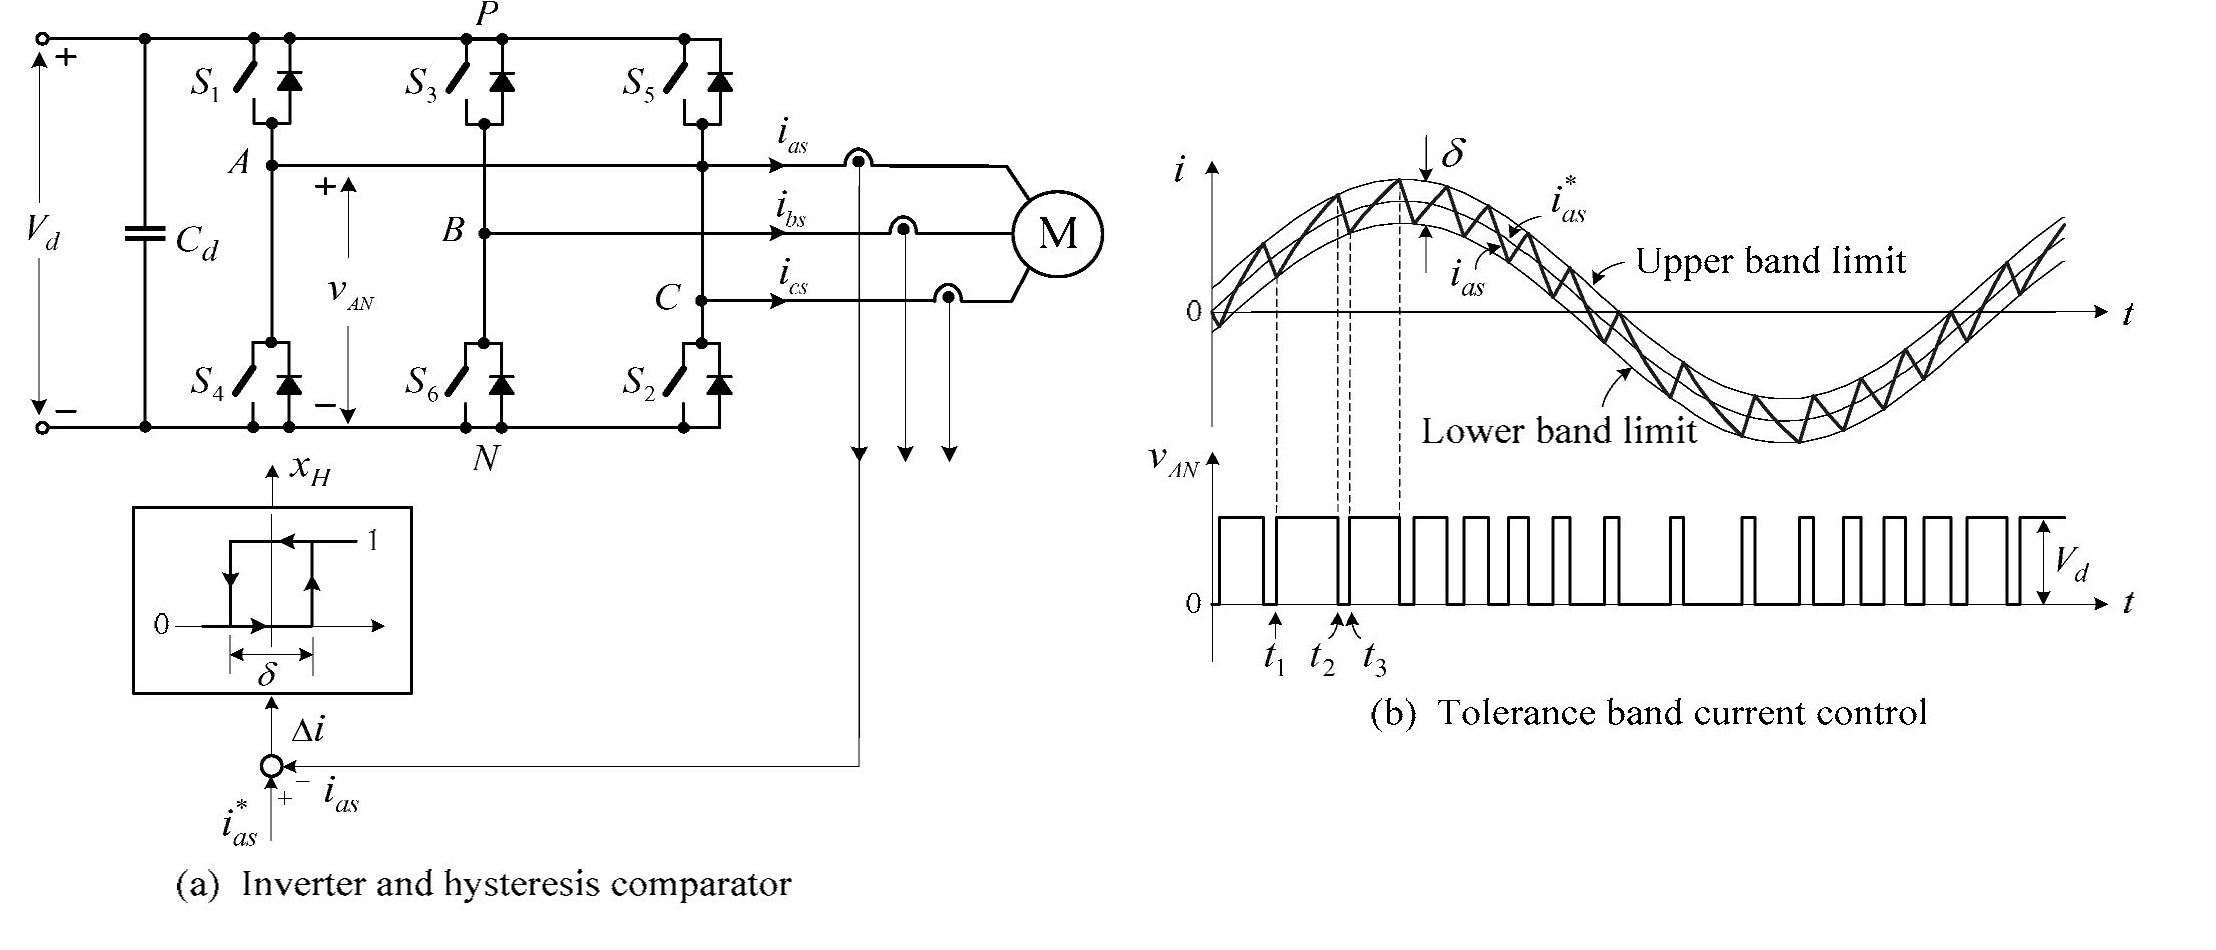
\includegraphics[scale=0.8]{graficos/img17.jpg}
\caption{Figura 14.5-5: Inversor de fuente de voltaje regulado por corriente.}
\end{figure}
\FloatBarrier

El principio de funcionamiento del VSI regulado por corriente se ilustra en la Fig. 14.5-5, donde se muestra el control de solo una de las tres corrientes de fase. La corriente de salida del inversor $i_{as}$ se mide y se compara con su referencia $i_{as}^*$. Su diferencia $\Delta i$ se envía a un comparador de histéresis. La salida del comparador $x_H$ es lógica '1' o '0', con base en la cual se generan señales de compuerta para los interruptores $S_1$ y $S_4$. El comparador de histéresis tiene una banda de tolerancia de $\delta$.

\clearpage
Supongamos que la corriente de referencia $i_{as}^*$ es sinusoidal como se ilustra en la Fig. 14.5-5b. La corriente de salida del inversor $i_{as}$ está confinada dentro de los límites superior e inferior establecidos por $\delta$. Suponiendo que $x_H$ se convierte en lógica '1' en el instante de tiempo $t_1$, $S_1$ se enciende y $S_4$ se apaga. El voltaje terminal del inversor $v_{AN}$ es igual al voltaje de corriente continua $V_d$, causando que $i_{as}$ aumente. La tasa de aumento de corriente está determinada principalmente por $V_d$, los parámetros del motor y su fuerza contraelectromotriz. Cuando $i_{as}$ alcanza su límite superior de banda en $t_2$, $x_H$ se convierte en lógica '0', lo que lleva al apagado de $S_1$ y al encendido de $S_4$. El $v_{AN}$ resultante es cero, causando que $i_{as}$ disminuya. Cuando $i_{as}$ alcanza el límite inferior de banda en $t_3$, $x_H$ = '0', $v_{AN}$ = $V_d$ y $i_{as}$ comienza a aumentar de nuevo. Como resultado, $i_{as}$ se mantiene dentro de los límites superior e inferior de la banda. Para hacer que $i_{as}$ siga su referencia $i_{as}^*$ más de cerca con menos armónicos de conmutación, se puede reducir el ancho de banda $\delta$. Sin embargo, esto se logra a expensas de una mayor frecuencia de conmutación.

Para un $\delta$ y $V_d$ dados, la frecuencia de conmutación del inversor puede variar con los parámetros del motor. Esto se considera como una desventaja importante del inversor regulado por corriente con control de banda de tolerancia. Cuando el inversor utiliza otras técnicas de modulación como SPWM y SVM, su frecuencia de conmutación está establecida por el esquema de modulación, independientemente de los parámetros del motor.

\begin{figure}[ht]
\centering
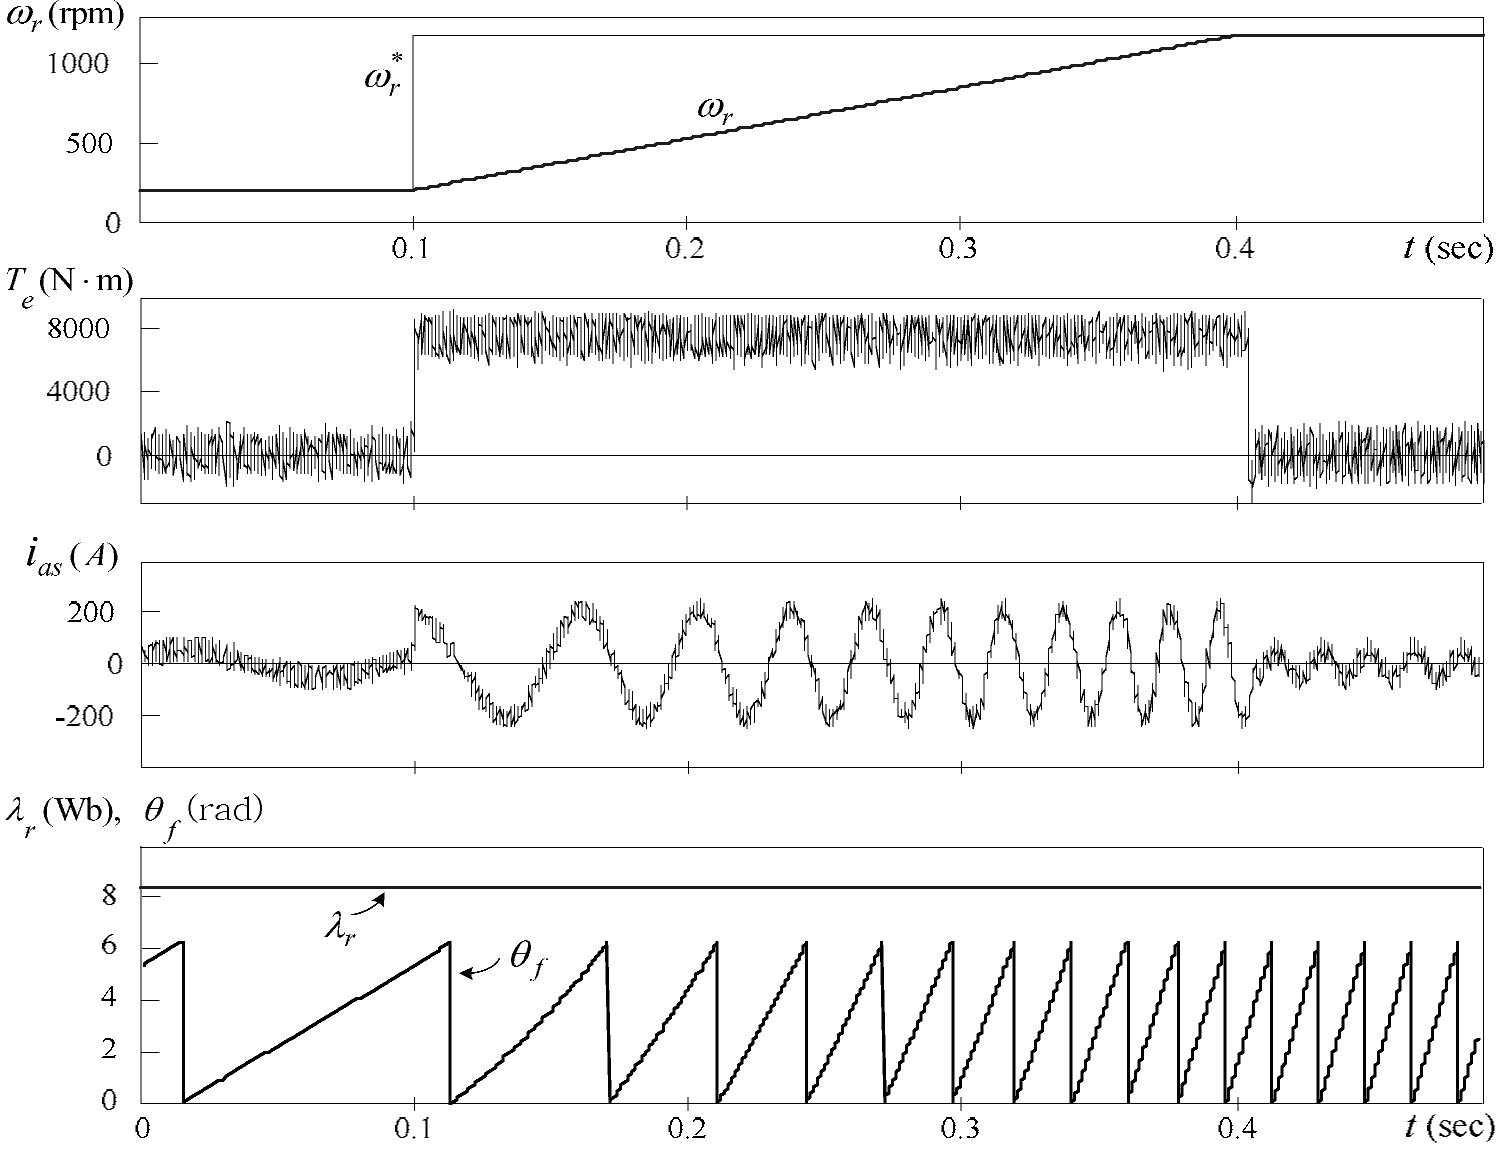
\includegraphics[scale=0.8]{graficos/img18.jpg}
\caption{Figura 14.5-6: Formas de onda simuladas para un drive de motor de inducción con esquema FOC directo.}
\end{figure}
\FloatBarrier

La Figura 14.5-6 muestra las formas de onda simuladas para un drive de motor de inducción utilizando el esquema FOC directo. El diagrama de bloques del sistema de drive se muestra en la Fig. 14.5-4, donde no se muestra el lazo de control de velocidad. Los datos de la placa de características del motor y los parámetros se enumeran en la Tabla 14.5-1.

La banda de tolerancia $\delta$ del comparador de histéresis se ajusta de manera que la frecuencia de conmutación del inversor sea de alrededor de 600 Hz. La referencia de flujo del rotor $\lambda_r^*$ se establece en su valor nominal de 8.35 Wb. El par máximo se limita a su valor nominal de 7490 N·m durante los transitorios del motor.

El motor opera inicialmente a una velocidad del rotor de $n_r = 200$ rpm. La referencia de velocidad $n_r^*$ tiene un aumento de paso de 200 rpm a la velocidad nominal del rotor de 1189 rpm en el instante de tiempo $t = 0.1$ s. El motor acelera bajo la condición de no carga mientras su par se limita al valor nominal. El par contiene altos rizados debido a la baja frecuencia de conmutación. La corriente del estator $i_{as}$ aumenta a su valor nominal durante el transitorio. Cuando $n_r$ alcanza su referencia de 1189 rpm alrededor de $t = 0.4$ s, el $T_e$ promedio cae a cero, y $i_{as}$ se reduce a un valor que corresponde a la corriente de magnetización del motor. Debido al control desacoplado de flujo y par por el esquema FOC, la magnitud del flujo del rotor $\lambda_r$ se mantiene constante durante los transitorios. El ángulo de flujo del rotor $\theta_f$ también se muestra en la figura.

\section{Control Indirecto Orientado al Campo}

\begin{figure}[ht]
\centering
\caption{Tabla 14.5-1: Placa de Características del Motor y Parámetros.}
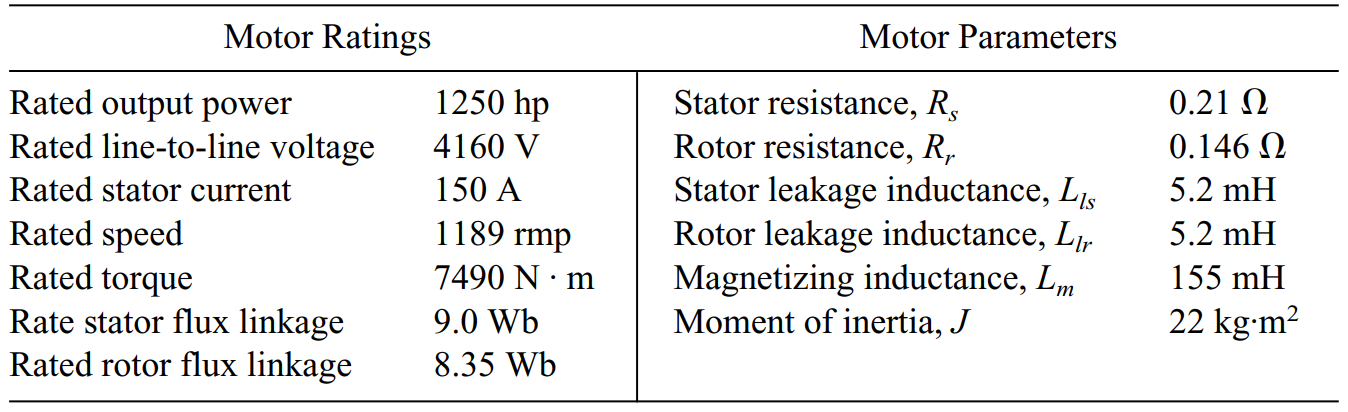
\includegraphics[scale=0.4]{graficos/tabla_14_5_1.png}
\end{figure}
\FloatBarrier

\begin{figure}[ht]
\centering
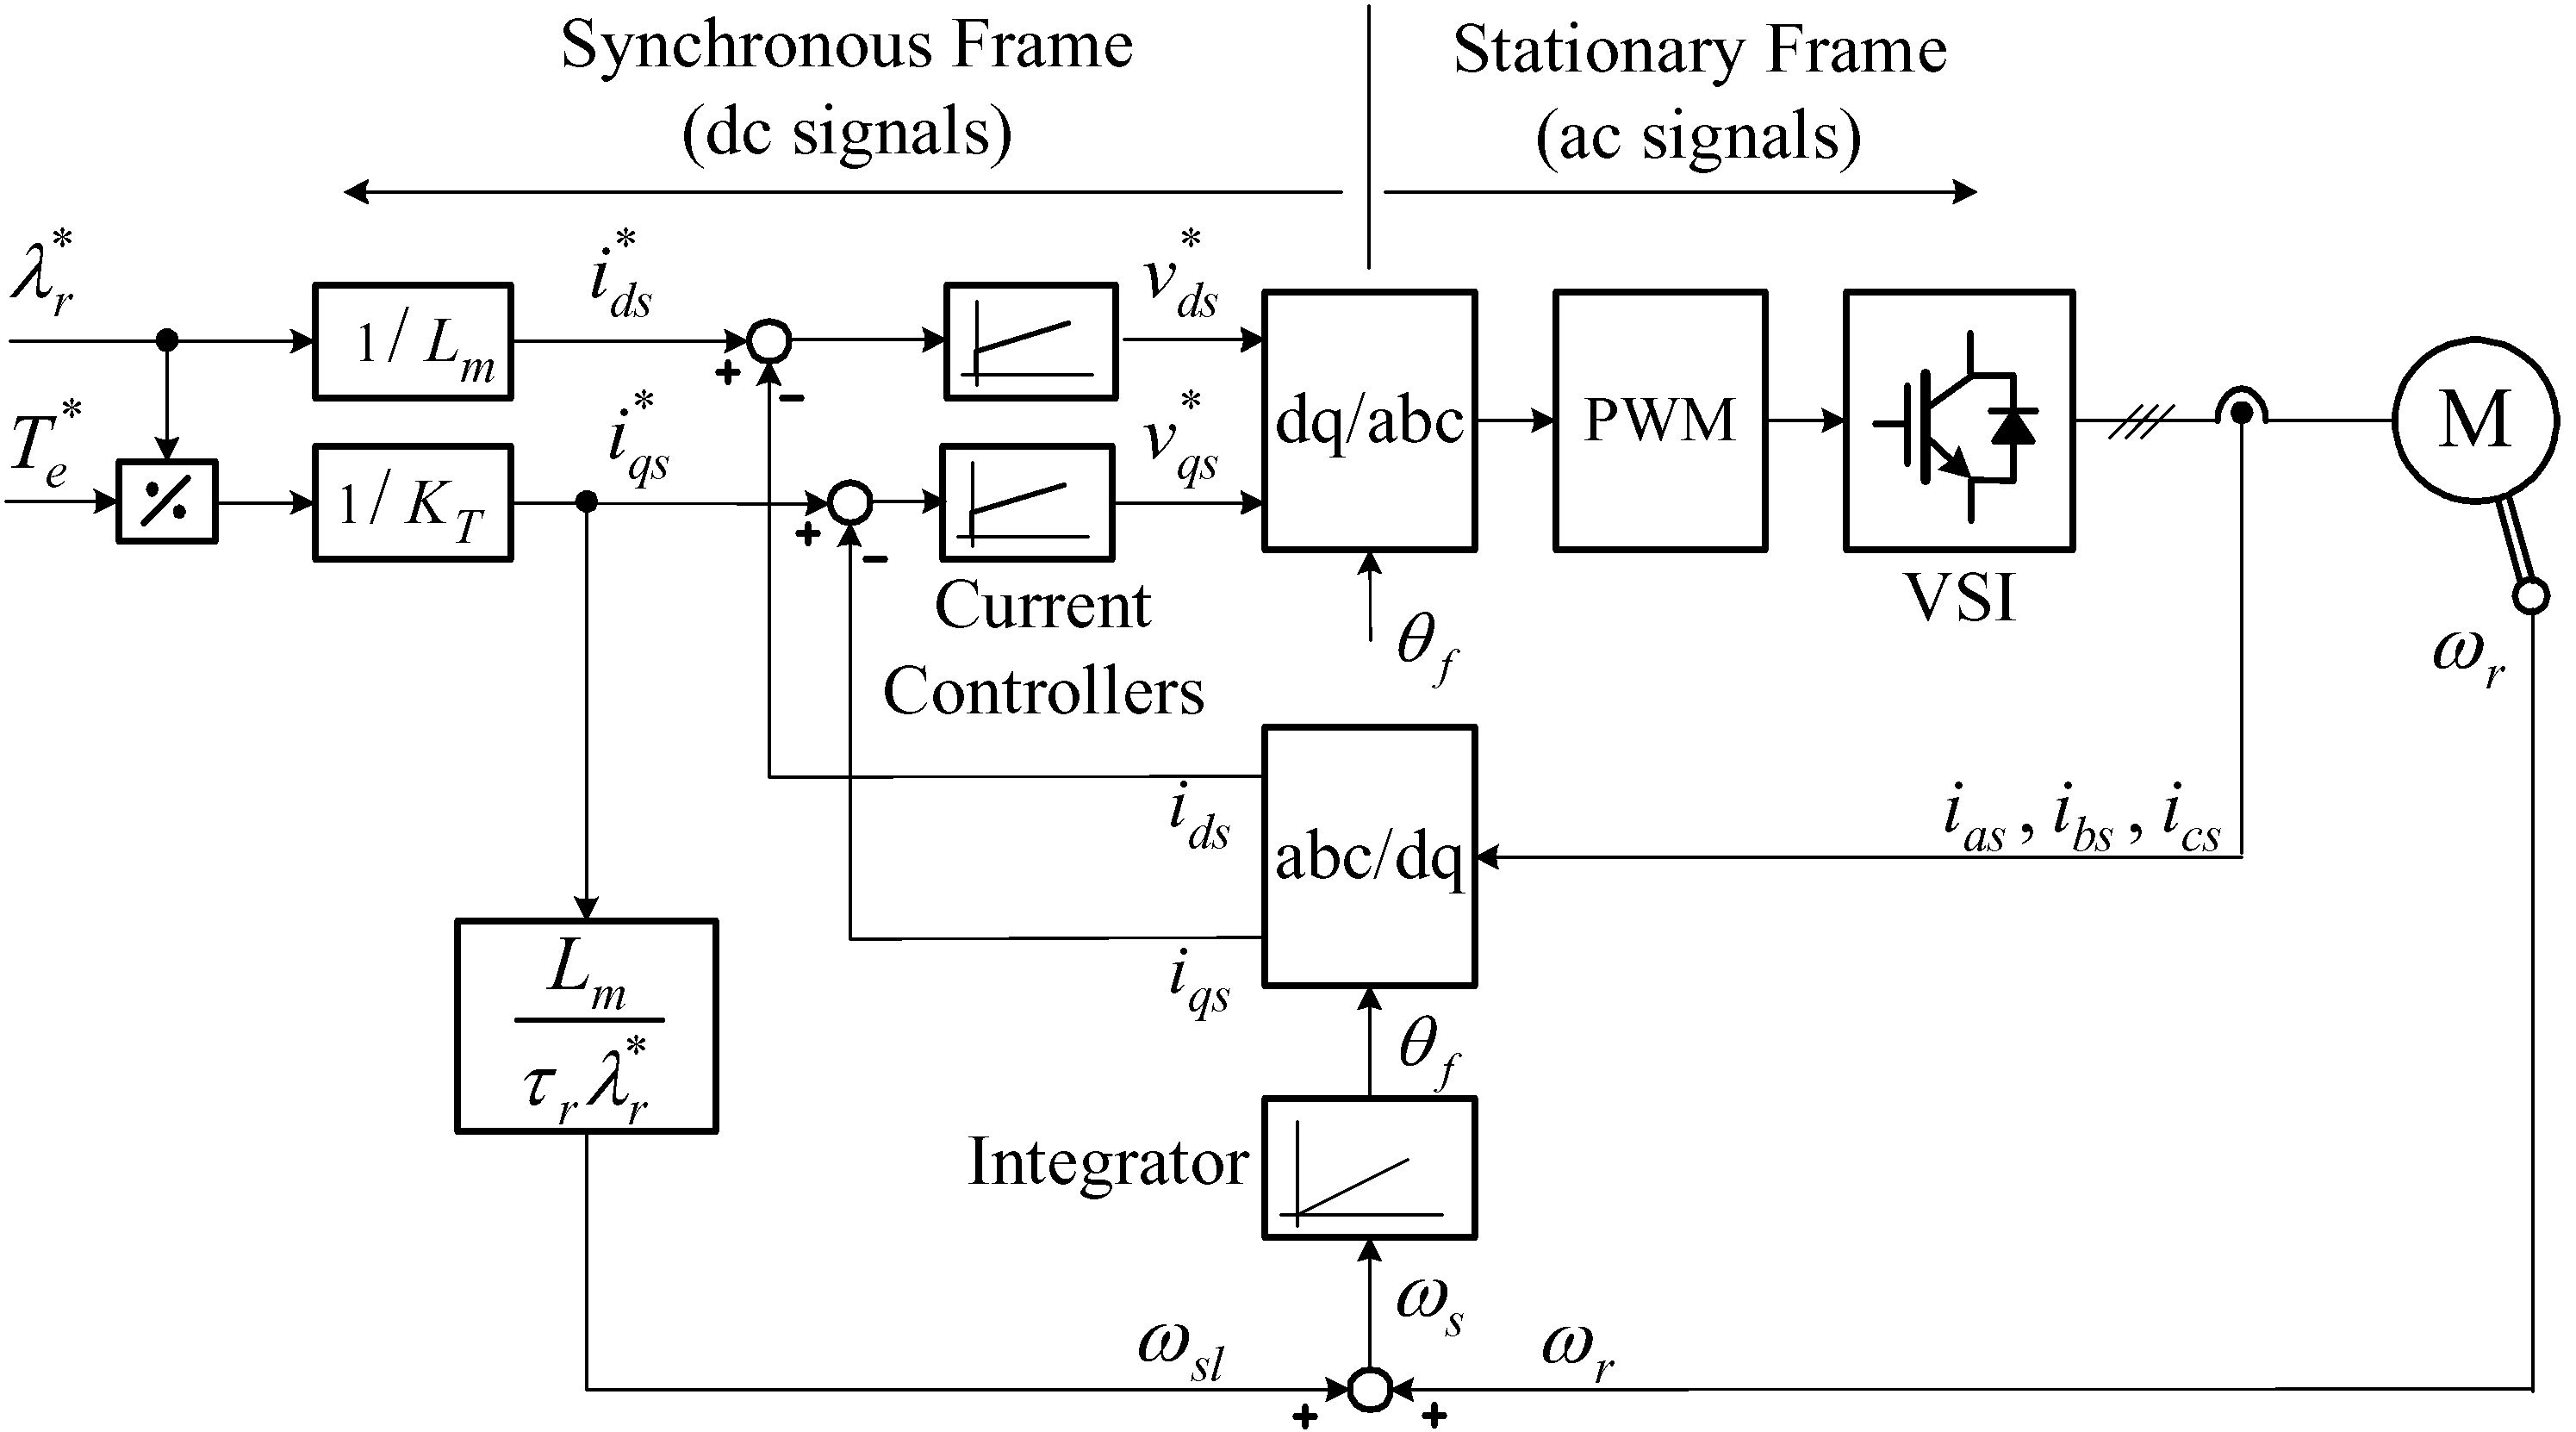
\includegraphics{graficos/img19.jpg}
\caption{Figura 14.6-1: Control indirecto orientado al campo con orientación al flujo del rotor.}
\end{figure}
\FloatBarrier

\clearpage
Se requiere un sensor digital de velocidad del rotor para los esquemas de control indirecto orientado al campo. El ángulo de flujo del rotor $\theta_f$ para la orientación del campo se obtiene a partir de la velocidad del rotor medida y el ángulo de deslizamiento calculado basado en los parámetros del motor. Un diagrama de bloques típico del FOC indirecto se muestra en la Fig. 14.6-1. Dado que la velocidad del rotor $\omega_r$ se mide directamente, el ángulo de flujo del rotor $\theta_f$ se puede encontrar a partir de

\begin{equation}
\theta_f = \int (\omega_r + \omega_{sl}) \, dt \tag{14.6-1}
\end{equation}

donde $\omega_{sl}$ es la frecuencia de deslizamiento angular.

La frecuencia de deslizamiento $\omega_{sl}$ se puede derivar del modelo del motor en el marco síncrono de la Fig. 14.3-2a, de la cual

\begin{equation}
p \lambda_r = -R_r \vec{i}_r - j \omega_{sl} \vec{\lambda}_r \tag{14.6-2}
\end{equation}

Sustituyendo la corriente del rotor

\begin{equation}
\vec{i}_r = \frac{1}{L_r} (\vec{\lambda}_r - L_m \vec{i}_s) \tag{14.6-3}
\end{equation}

en (14.6-2) se obtiene

\begin{equation}
p \vec{\lambda}_r = -\frac{R_r}{L_r} \left( \vec{\lambda}_r - L_m \vec{i}_s \right) - j \omega_{sl} \vec{\lambda}_r \tag{14.6-4}
\end{equation}

de donde

\begin{equation}
\vec{\lambda}_r (1 + \tau_r (p + j \omega_{sl})) = L_m \vec{i}_s \tag{14.6-5}
\end{equation}

donde $\tau_r$ es la constante de tiempo del rotor, definida por

\begin{equation}
\tau_r = \frac{L_r}{R_r} \tag{14.6-6}
\end{equation}

\clearpage
Descomponiendo (14.6-5) en los componentes de los ejes $dq$ y teniendo en cuenta la orientación del flujo del rotor ($j \lambda_{qr} = 0$ y $\lambda_{dr} = \lambda_r$), tenemos

\begin{equation}
\lambda_r (1 + p \tau_r) = L_m i_{ds} \tag{14.6-7}
\end{equation}

\begin{equation}
\omega_{sl} \tau_r \lambda_r = L_m i_{qs} \tag{14.6-7}
\end{equation}

de donde

\begin{equation}
\omega_{sl} = \frac{L_m}{\tau_r \lambda_r} i_{qs} \tag{14.6-8}
\end{equation}

Como se muestra en la Fig. 14.6-1, el flujo del rotor y el par se controlan por dos lazos de retroalimentación por separado. Basado en (14.6-7), la relación entre la referencia del flujo del rotor $\lambda_r^*$ y la referencia de corriente del eje d $i_{ds}^*$ se puede expresar como

\begin{equation}
i_{ds}^* = \frac{(1 + p \tau_r)}{L_m} \lambda_r^* \tag{14.6-9}
\end{equation}

Dado que $\lambda_r^*$ normalmente se mantiene constante durante la operación ($p \lambda_r^* = 0$), (14.6-9) se puede simplificar a

\begin{equation}
i_{ds}^* = \frac{1}{L_m} \lambda_r^* \tag{14.6-10}
\end{equation}

La referencia de corriente del eje q $i_{qs}^*$ se puede obtener a partir de la ecuación de par de (14.4-3):

\begin{equation}
i_{qs}^* = \frac{1}{K_T \lambda_r^*} T_e^* \tag{14.6-11}
\end{equation}

Para una $\lambda_r^*$ dada, la corriente de producción de par $i_{qs}^*$ es proporcional a $T_e^*$.

\clearpage
\section{FOC para Drives Alimentados por CSI}

\begin{figure}[ht]
\centering
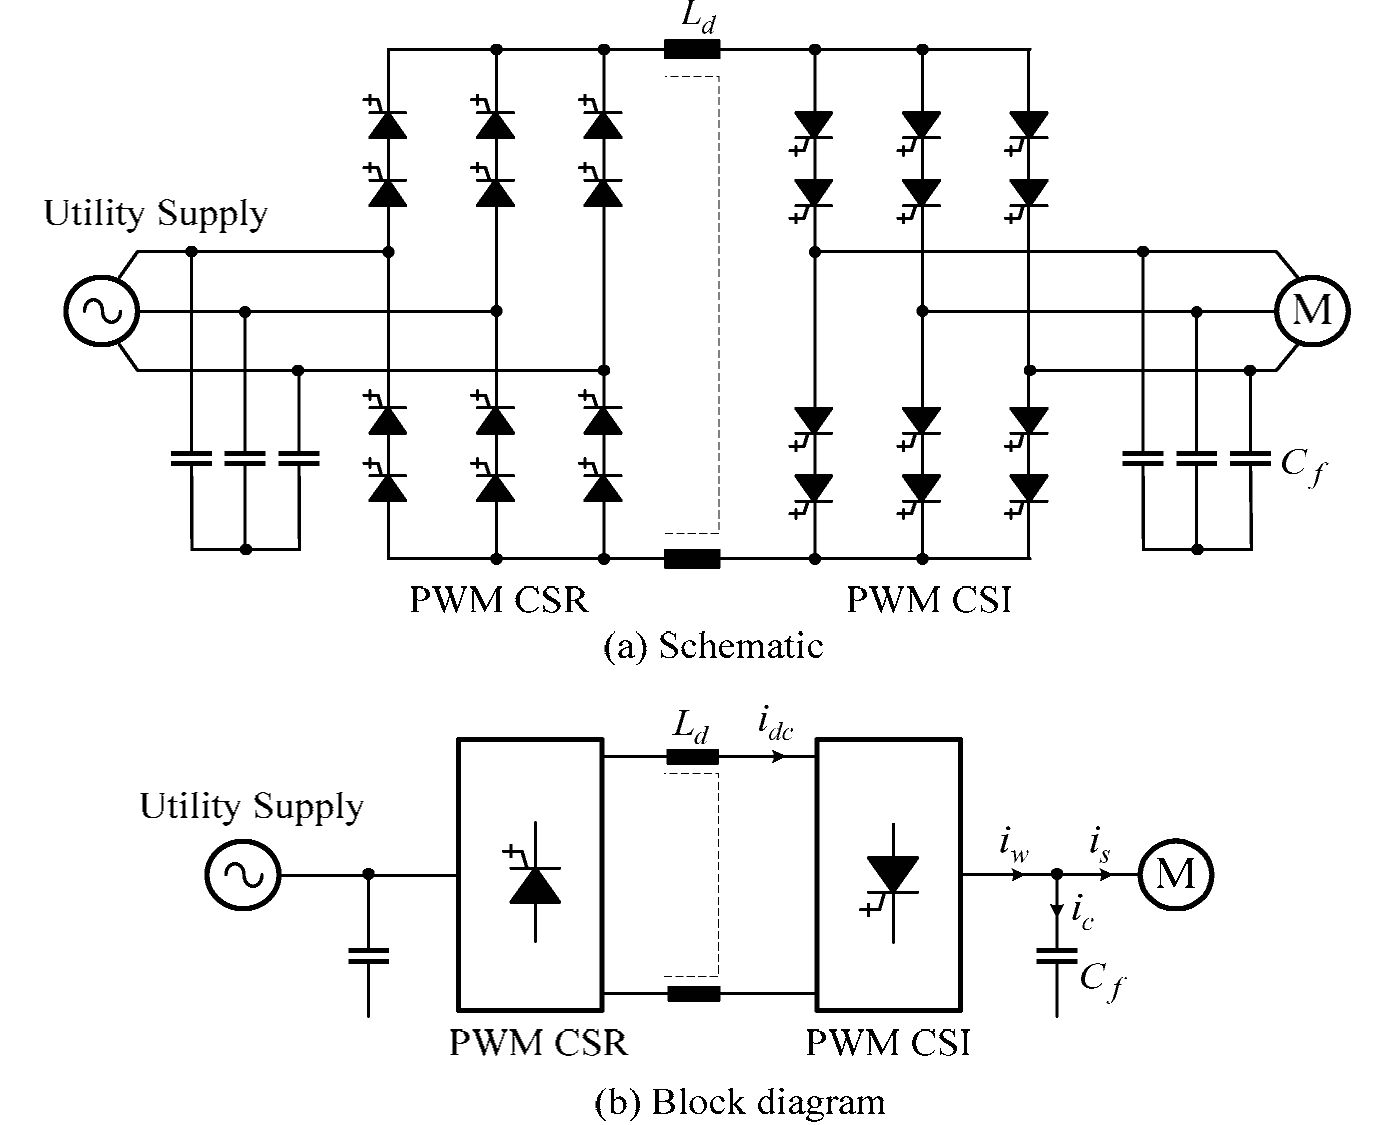
\includegraphics{graficos/img20.jpg}
\caption{Figura 14.7-1: Un drive basado en convertidor de fuente de corriente PWM.}
\end{figure}
\FloatBarrier

En los drives de MV alimentados por VSI, tanto el voltaje de salida del inversor como la frecuencia pueden ser controlados por su esquema PWM. Sin embargo, este no es el caso para el drive alimentado por CSI mostrado en la Fig. 14.7-1, donde la frecuencia de salida del inversor se controla por su esquema PWM, mientras que la corriente de salida del inversor $\vec{i}_w$ se ajusta por la corriente de corriente continua $i_{dc}$ del rectificador. Además, la corriente del estator $\vec{i}_s$ no es controlada directamente por $\vec{i}_w$ debido al condensador del filtro $C_f$. Por lo tanto, se requieren medidas adicionales para mantener la orientación del campo en los drives CSI.

\begin{figure}[ht]
\centering
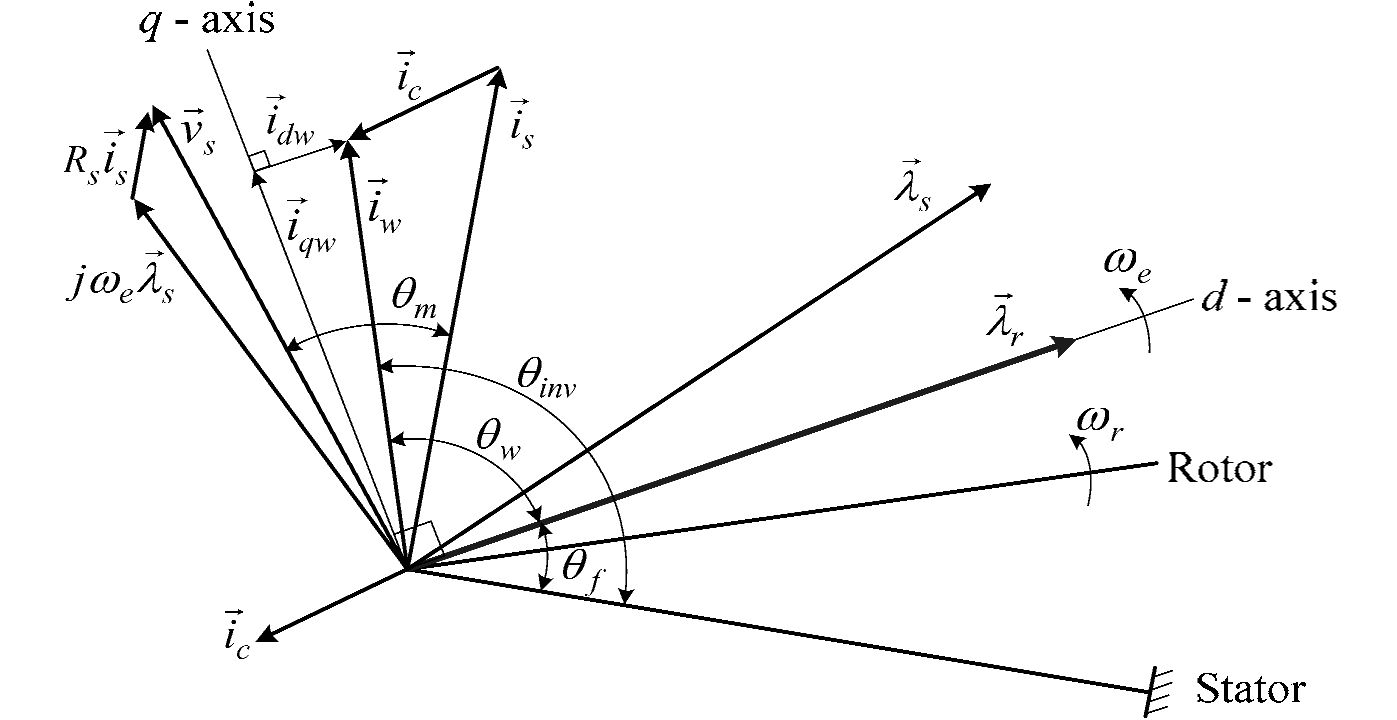
\includegraphics{graficos/img21.jpg}
\caption{Figura 14.7-2: Diagrama vectorial para un drive alimentado por CSI con orientación al flujo del rotor.}
\end{figure}
\FloatBarrier

La Figura 14.7-2 muestra el diagrama del vector espacial para el drive CSI con control orientado al flujo del rotor. El eje $d$ del marco de referencia síncrono está alineado con el vector de flujo del rotor $\vec{\lambda}_r$. El vector de flujo del estator $\vec{\lambda}_s$ adelanta al flujo del rotor $\vec{\lambda}_r$ por un pequeño ángulo debido a las inductancias de fuga. El voltaje del estator $\vec{v}_s$ es la suma del voltaje de velocidad $j\omega \vec{\lambda}_s$ y la caída de voltaje de la resistencia del estator $R_s \vec{i}_s$. La corriente del estator $\vec{i}_s$ está retrasada con respecto a $\vec{v}_s$ por $\theta_{m}$, que es el ángulo del factor de potencia del motor. La corriente del condensador $\vec{i}_c$ adelanta a $\vec{v}_s$ por $\pi/2$. La corriente PWM del inversor $\vec{i}_w$ es una suma vectorial de $\vec{i}_s$ y $\vec{i}_c$, y su ángulo con respecto a $\vec{\lambda}_r$ es $\theta_{w}$. El ángulo de disparo del inversor es

\begin{equation}
\theta_{inv} = \theta_{w} + \theta_{f} \tag{14.7-1}
\end{equation}

donde $\theta_{f}$ es el ángulo de flujo del rotor para la orientación del campo. Cuando el drive opera en estado estacionario, $\theta_{w}$ es constante ya que tanto $\vec{i}_w$ como $\vec{\lambda}_r$ están en el marco de referencia síncrono, mientras que $\theta_{f}$ y $\theta_{inv}$ varían periódicamente entre cero y $2\pi$.

\begin{figure}[ht]
\centering
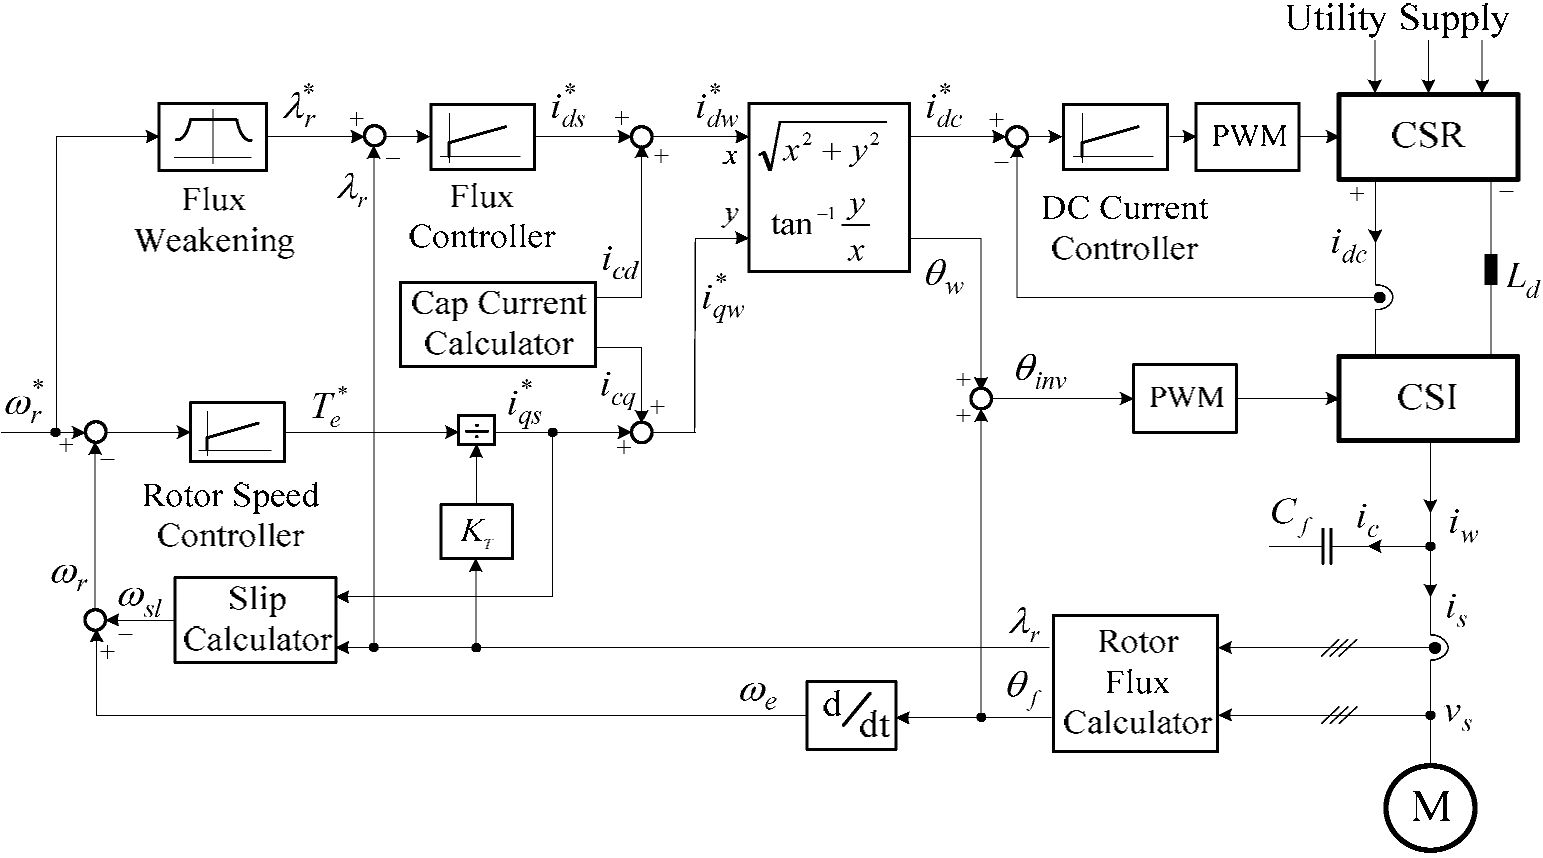
\includegraphics{graficos/img22.jpg}
\caption{Figura 14.7-3: Diagrama de bloques simplificado para un drive alimentado por CSI usando el esquema FOC directo.}
\end{figure}
\FloatBarrier

La Figura 14.7-3 muestra un diagrama de bloques simplificado para el drive alimentado por CSI con control orientado al campo directo. El esquema FOC se implementa con tres lazos de control de retroalimentación, uno para la velocidad del rotor $\omega_r$, uno para el flujo del rotor $\lambda_r$ y otro para la corriente de corriente continua $i_{dc}$. La velocidad del rotor $\omega_r$ se obtiene por $\omega_r = \omega_e - \omega_{sl}$ donde $\omega_e = d\theta_f / dt$ y $\omega_{sl}$ se puede calcular mediante (14.6-8).

La referencia de corriente del estator en el eje $q$ (producción de par) $i_{qs}^*$ y la referencia de corriente en el eje $d$ (producción de flujo) $i_{ds}^*$ se generan de la misma manera que se muestra en la Fig. 14.5-1. Las referencias de corriente PWM del inversor en el eje $dq$ se pueden expresar como

\begin{equation}
i_{dw}^* = i_{cd} + i_{ds}^* \tag{14.7-2}
\end{equation}

\begin{equation}
i_{qw}^* = i_{cq} + i_{qs}^* \tag{14.7-3}
\end{equation}

donde $i_{cd}$ y $i_{cq}$ son las corrientes del condensador en el eje $dq$, dadas por

\begin{equation}
i_{cd} = (p v_{ds} - \omega_e v_{qs}) C_f \tag{14.7-4}
\end{equation}

\begin{equation}
i_{cq} = (p v_{qs} + \omega_e v_{ds}) C_f \tag{14.7-5}
\end{equation}

El primer término en el lado derecho de la ecuación representa la corriente transitoria del condensador, y el segundo término es la corriente en estado estacionario. Para reducir la sensibilidad y el ruido causado por los términos derivados $(p v_{ds}$ y $p v_{qs})$, se puede despreciar el efecto de la respuesta transitoria del condensador en el rendimiento dinámico del drive. La ecuación (14.7-3) se puede simplificar a

\begin{equation}
i_{cd} = \omega_e v_{qs} C_f \tag{14.7-6}
\end{equation}

\begin{equation}
i_{cq} = \omega_e v_{ds} C_f \tag{14.7-7}
\end{equation}

para su uso en el Calculador de Corriente del Condensador en la Fig. 14.7-3.

Dado que la magnitud de $i_w$ es proporcional a la corriente de corriente continua, la referencia de corriente de corriente continua se puede encontrar a partir de

\begin{equation}
i_{dc}^* = \sqrt{(i_{dw}^*)^2 + (i_{qw}^*)^2} \tag{14.7-8}
\end{equation}

El ángulo de disparo del inversor $\theta_{inv}$ es la suma de $\theta_f$ y $\theta_w$, donde $\theta_f$ se puede obtener del Calculador de Flujo del Rotor en la Fig. 14.5-3 y $\theta_w$ se puede determinar mediante

\begin{equation}
\theta_w = \tan^{-1} (i_{qw}^* / i_{dw}^*) \tag{14.7-9}
\end{equation}

Varios esquemas PWM, como SHE, TPWM y SVM presentados en los Capítulos 10 y 11, se pueden emplear para los bloques PWM en la Fig. 14.7-3.

\section{Control Directo de Par}
El control directo de par (DTC) es uno de los esquemas de control avanzado para los drives de corriente alterna (ac) [5-7]. Se caracteriza por su algoritmo de control simple, fácil implementación digital y operación robusta [8, 9]. En esta sección se introduce el principio del esquema DTC y se proporcionan resultados de simulación.

\subsection{Principio del Control Directo de Par}
El par electromagnético desarrollado por un motor de inducción puede expresarse de varias maneras, una de las cuales es

\begin{equation}
T_e = \frac{3P}{2} \frac{L_m}{\sigma L_s L_r} \lambda_s \lambda_r \sin \theta_r \tag{14.8-1}
\end{equation}

donde $\theta_r$ es el ángulo entre el vector de flujo del estator $\vec{\lambda_s}$ y el vector de flujo del rotor $\vec{\lambda_r}$, conocido como ángulo de par. Esta ecuación indica que $T_e$ puede ser controlado directamente por $\theta_r$.

La principal variable a controlar en el esquema DTC es el vector de flujo del estator $\vec{\lambda_s}$. Refiriéndose al modelo del motor de inducción de la Fig. 14.3-2b, $\vec{\lambda_s}$ relaciona el vector de voltaje del estator $\vec{v_s}$ mediante

\begin{equation}
p \vec{\lambda_s} = \vec{v_s} - R_s \vec{i_s} \tag{14.8-2}
\end{equation}

La ecuación muestra que la derivada de $\vec{\lambda_s}$ reacciona instantáneamente a los cambios en $\vec{v_s}$. Como se discutió en el Capítulo 6, el voltaje del estator $\vec{v_s}$, que es el voltaje de salida del inversor, puede ser controlado por el vector de referencia $\vec{V_{ref}}$` en la modulación de vector espacial. Dado que $\vec{V_{ref}}$` se sintetiza por los vectores de voltaje estacionarios del inversor, una selección adecuada de los vectores estacionarios puede hacer que la magnitud y el ángulo de $\vec{\lambda_s}$ sean ajustables.

\begin{figure}[ht]
\centering
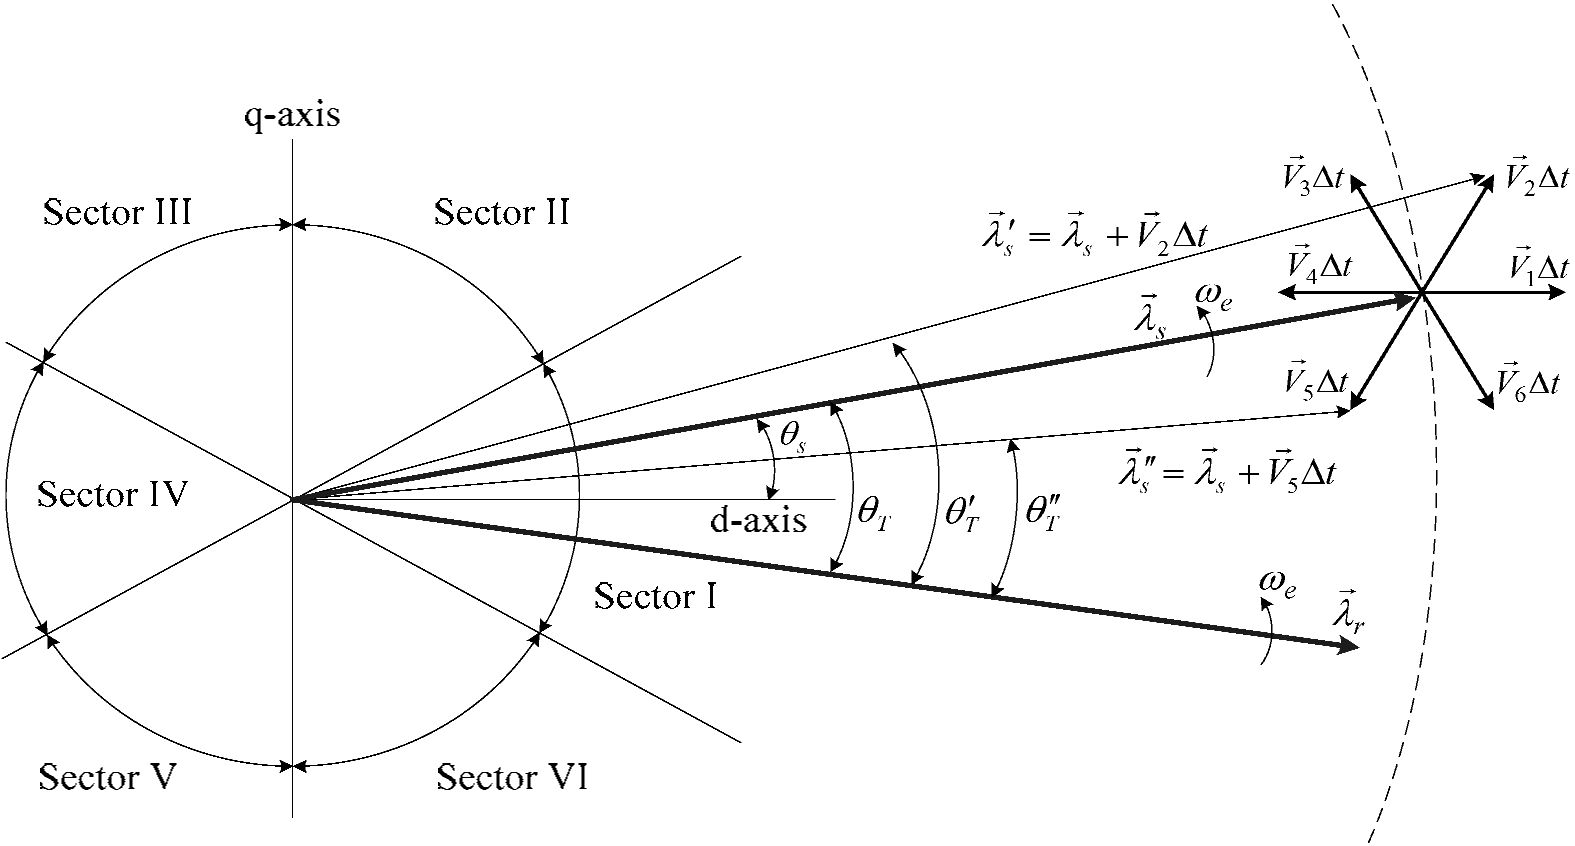
\includegraphics[scale=0.9]{graficos/img23.jpg}
\caption{Figura 14.8-1: Principio del control directo de par.}
\label{fig:14.8-1}
\end{figure}
\FloatBarrier

La Figura 14.8-1 muestra el principio del control directo de par para un drive de motor de inducción alimentado por VSI de dos niveles. El plano del eje $dq$ para el flujo del estator $\vec{\lambda_s}$ se divide en seis sectores I a VI. El flujo del estator $\vec{\lambda_s}$ en la figura cae en el sector I, y su ángulo $\theta_s$ se refiere al eje d del marco de referencia estacionario. El vector de flujo del rotor $\vec{\lambda_r}$ se retrasa con respecto a $\vec{\lambda_s}$ por $\theta_r$.

Vamos a examinar el impacto de los vectores de voltaje estacionarios $\vec{V_0}$ a $\vec{V_6}$ en $\vec{\lambda_s}$ y $\theta_r$. Supongamos que $\vec{\lambda_s}$ y $\theta_r$ en la Fig. 14.8-1 son el vector de flujo del estator inicial y el ángulo de par. Cuando se selecciona el vector de voltaje $\vec{V_2}$, el vector de flujo del estator se convertirá en $\vec{\lambda_s}' = \vec{\lambda_s} + \vec{V_2}\Delta t$ después de un corto intervalo de tiempo $\Delta t$, lo que lleva a un aumento en la magnitud del flujo ($\lambda_s' > \lambda_s$) y el ángulo de par ($\theta_r' > \theta_r$). Si se selecciona el vector de voltaje $\vec{V_5}$, $\vec{\lambda_s}$ cambiará a $\vec{\lambda_s}'' = \vec{\lambda_s} + \vec{V_5}\Delta t$, causando una disminución en la magnitud del flujo ($\lambda_s'' < \lambda_s$) y el ángulo de par ($\theta_r'' < \theta_r$). De manera similar, la selección de $\vec{V_3}$ y $\vec{V_6}$ puede hacer que una variable aumente y la otra disminuya. Por lo tanto, $\lambda_s$ y $\theta_r$ pueden ser controlados por separado mediante la selección adecuada de los vectores de voltaje del inversor.

Cabe señalar que los cambios en $\vec{v_s}$ tienen un impacto mucho menor en $\vec{\lambda_r}$ durante un corto intervalo de tiempo $\Delta t$ debido a la gran constante de tiempo del rotor. Por lo tanto, se asume en el análisis anterior que el vector de flujo del rotor $\vec{\lambda_r}$ se mantiene constante durante $\Delta t$.

\subsection{Lógica de Conmutación}

\begin{figure}[ht]
\centering
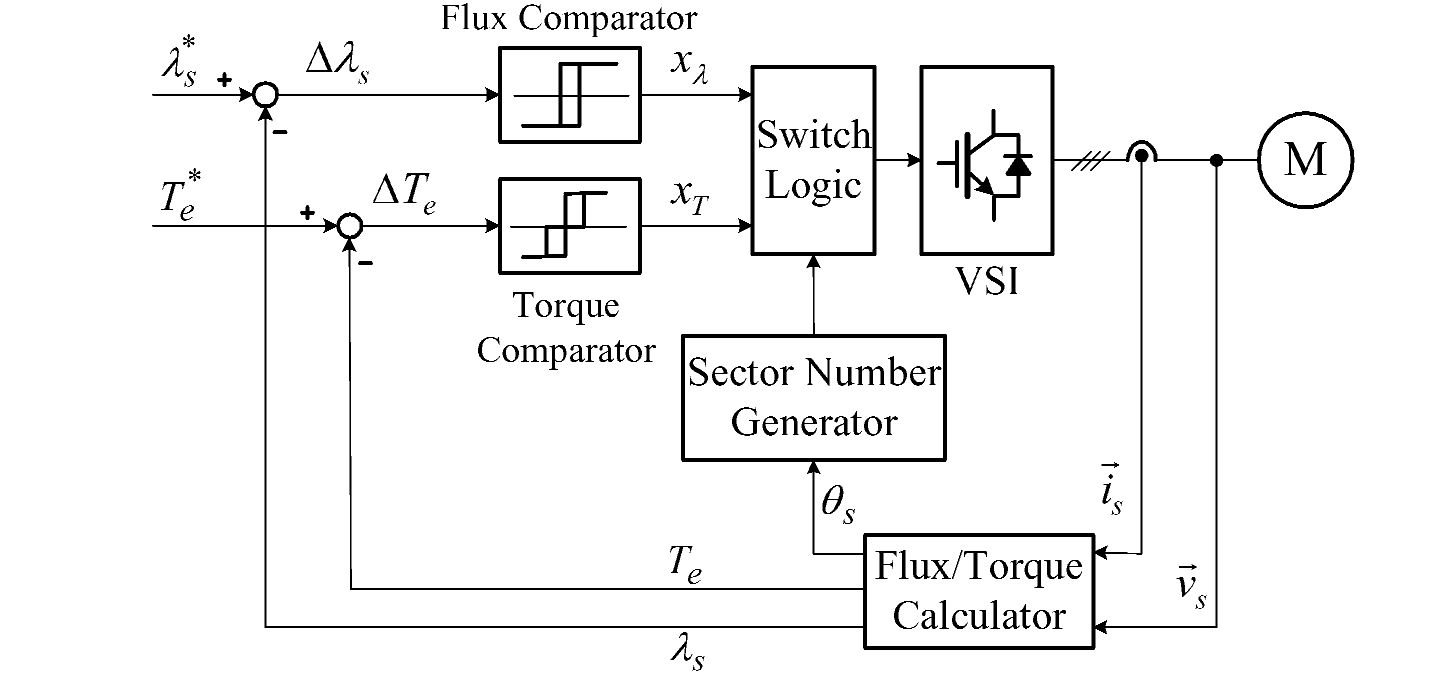
\includegraphics{graficos/img24.jpg}
\caption{Figura 14.8-2: Diagrama de bloques del esquema de control directo de par.}
\label{fig:14.8-2}
\end{figure}
\FloatBarrier

La Figura 14.8-2 muestra un diagrama de bloques típico de un drive de motor de inducción basado en DTC, donde no se muestra el lazo de retroalimentación de velocidad del rotor para mayor simplicidad. Similar a los esquemas FOC, el flujo del estator y el par electromagnético se controlan por separado para lograr un rendimiento dinámico superior. La referencia de flujo del estator $\lambda_s^*$ se compara con el flujo del estator calculado $\lambda_s$, y el error $\Delta \lambda_s$ se envía al Comparador de Flujo. La referencia de par $T_e^*$ se compara con el par calculado $T_e$, y su diferencia $\Delta T_e$ es la entrada del Comparador de Par. La salida de los comparadores de flujo y par ($\chi_\lambda$ y $\chi_T$) se envían a la unidad de Lógica de Conmutación para la selección adecuada de los vectores de voltaje (estados de conmutación) del inversor.

\begin{figure}[ht]
\centering
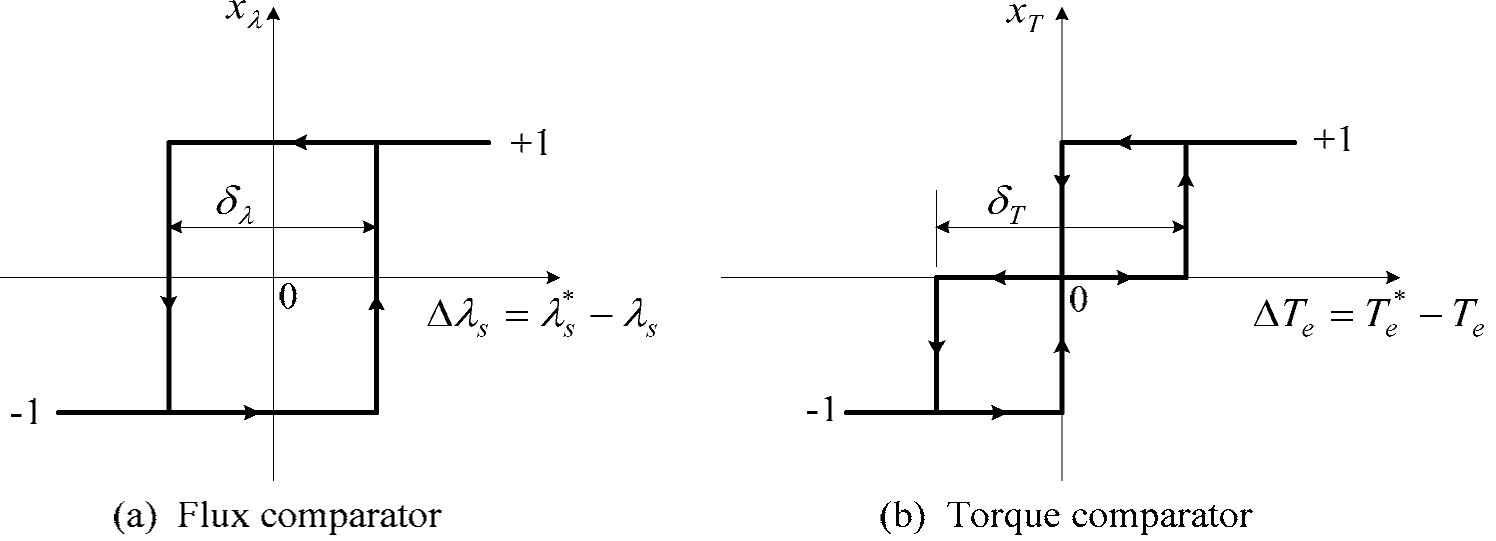
\includegraphics{graficos/img25.jpg}
\caption{Figura 14.8-3: Características de los comparadores de histéresis.}
\label{fig:14.8-3}
\end{figure}
\FloatBarrier

Ambos comparadores de flujo y par son de tipo histéresis (banda de tolerancia), cuyas características de transferencia se muestran en la Fig. 14.8-3. El comparador de flujo tiene dos niveles de salida ($\chi_\lambda = +1$ y $-1$) mientras que el comparador de par tiene tres niveles de salida ($\chi_T = +1, 0$ y $-1$), donde "+1" solicita un aumento en $\lambda_s$ o $\theta_r$, "-1" demanda una disminución en $\lambda_s$ o $\theta_r$, y "0" significa que no hay cambios. La banda de tolerancia para los comparadores de flujo y par es $\delta_\lambda$ y $\delta_T$, respectivamente.

\begin{figure}[ht]
\centering
\caption{Tabla 14.8-1: Lógica de Conmutación para $\vec{\lambda_s}^*$ Rotando en Sentido Antihorario.}
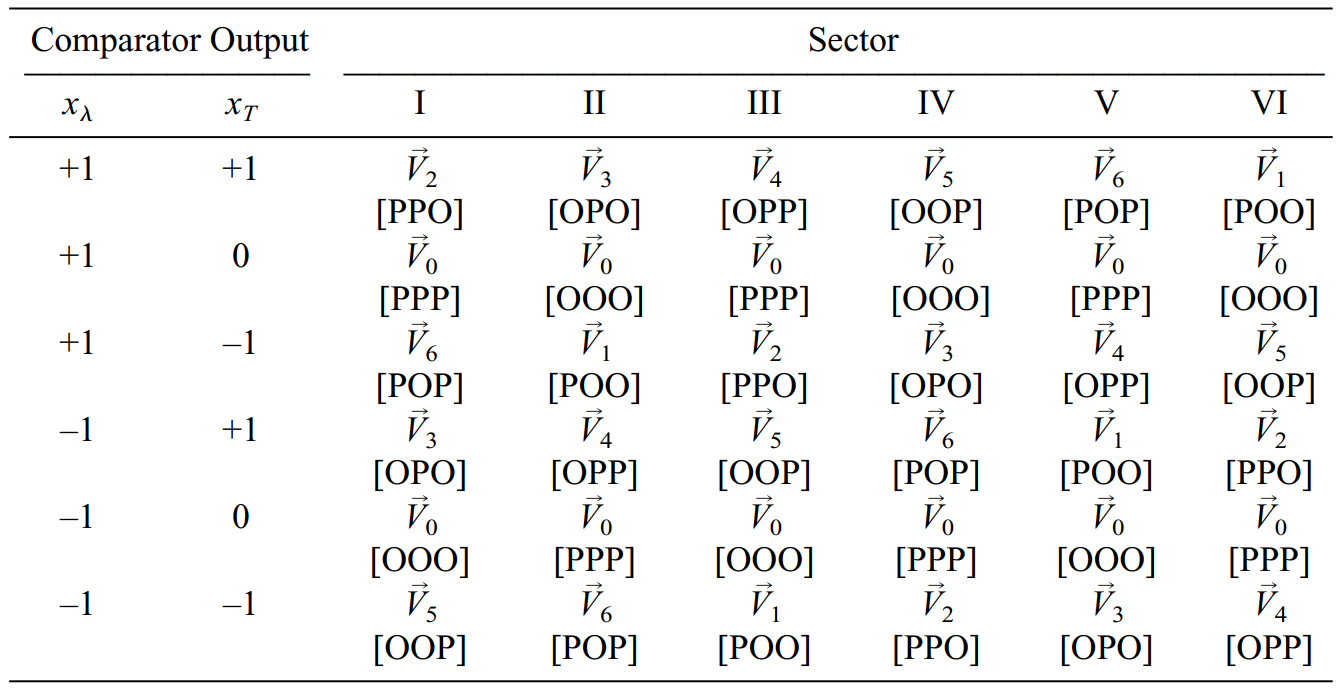
\includegraphics[scale=0.4]{graficos/tabla_14_8_1.png}
\label{tab:14.8-1}
\end{figure}
\FloatBarrier

La Tabla 14.8-1 proporciona la lógica de conmutación para la referencia de flujo del estator $\vec{\lambda_s}^*$ rotando en sentido antihorario. Las variables de entrada son $\chi_\lambda$, $\chi_T$ y el número de sector, y las variables de salida son los vectores de voltaje del inversor. La salida de los comparadores decide qué vector de voltaje debe seleccionarse. Suponiendo que $\vec{\lambda_s}^*$ está en el sector I, la salida del comparador $\chi_\lambda = \chi_T = +1$ significa un aumento en $\lambda_s$ y $T_e$. El vector de voltaje $\vec{V_2}$ puede ser seleccionado de la tabla. Esta selección hará que tanto $\lambda_s$ como $\theta_r$ aumenten como se muestra en la Fig. 14.8-1.

Cuando la salida del comparador de par $\chi_T$ es cero (no es necesario ajustar $T_e$), se puede seleccionar el vector cero $\vec{V_0}$. El uso alternativo de los estados de conmutación [OOO] y [PPP] para $\vec{V_0}$ en la tabla de conmutación puede ayudar a reducir la frecuencia de conmutación del dispositivo. Por ejemplo, cuando $\chi_T$ cambia entre '+1' y '0' o entre '0' y '-1', los estados cero en la tabla aseguran que solo dos interruptores estén involucrados durante la transición, uno siendo encendido y el otro apagado.

\begin{figure}[ht]
\centering
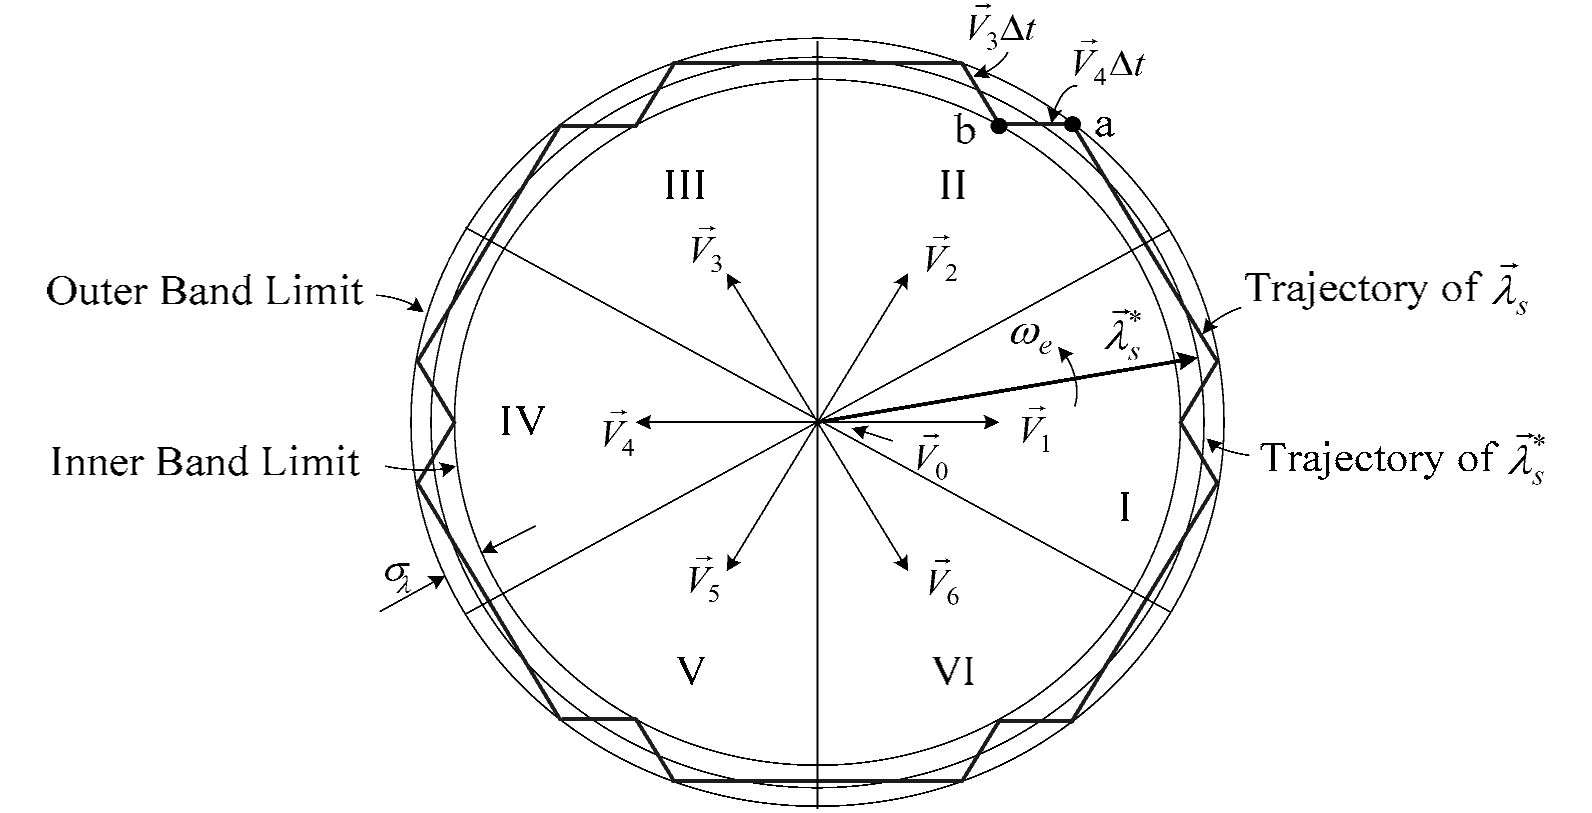
\includegraphics{graficos/img26.jpg}
\caption{Figura 14.8-4: Trayectorias del flujo del estator $\vec{\lambda_s}$ y su referencia $\vec{\lambda_s}^*$ con $\chi_T = 1$.}
\label{fig:14.8-4}
\end{figure}
\FloatBarrier

\clearpage
El funcionamiento del control directo de par se puede explicar aún más con el diagrama de trayectorias del flujo del estator de la Fig. 14.8-4. Supongamos que el vector de referencia $\vec{\lambda_s}^*$ gira en sentido antihorario durante la aceleración de la velocidad del rotor y la salida del comparador de par es $\chi_T = +1`$. Cuando $\lambda_s$ alcanza el límite de la banda exterior en el punto $a$ en el sector II, la salida del comparador de flujo $\chi_\lambda$ se convierte en '-1', y se selecciona el vector $\vec{V_4}$ de la tabla de conmutación, lo que provocará una disminución en $\lambda_s$. Cuando $\lambda_s$ alcanza el límite de la banda interior en el punto $b$, $\chi_\lambda$ se convierte en +1, y se selecciona el vector $\vec{V_3}$, aumentando $\lambda_s$. La trayectoria de $\vec{\lambda_s}$ en la figura no es muy suave debido al ancho amplio de la banda de tolerancia $\delta_\lambda$, lo que se traduce en un alto rizado del flujo del estator y una baja frecuencia de conmutación. La calidad de la forma de onda del flujo del estator se puede mejorar reduciendo $\delta_\lambda$, pero se logra a expensas de un aumento en la frecuencia de conmutación.

\begin{figure}[ht]
\centering
\caption{Tabla 14.8-2: Lógica de Conmutación para el Flujo del Estator Rotando en Sentido Horario.}
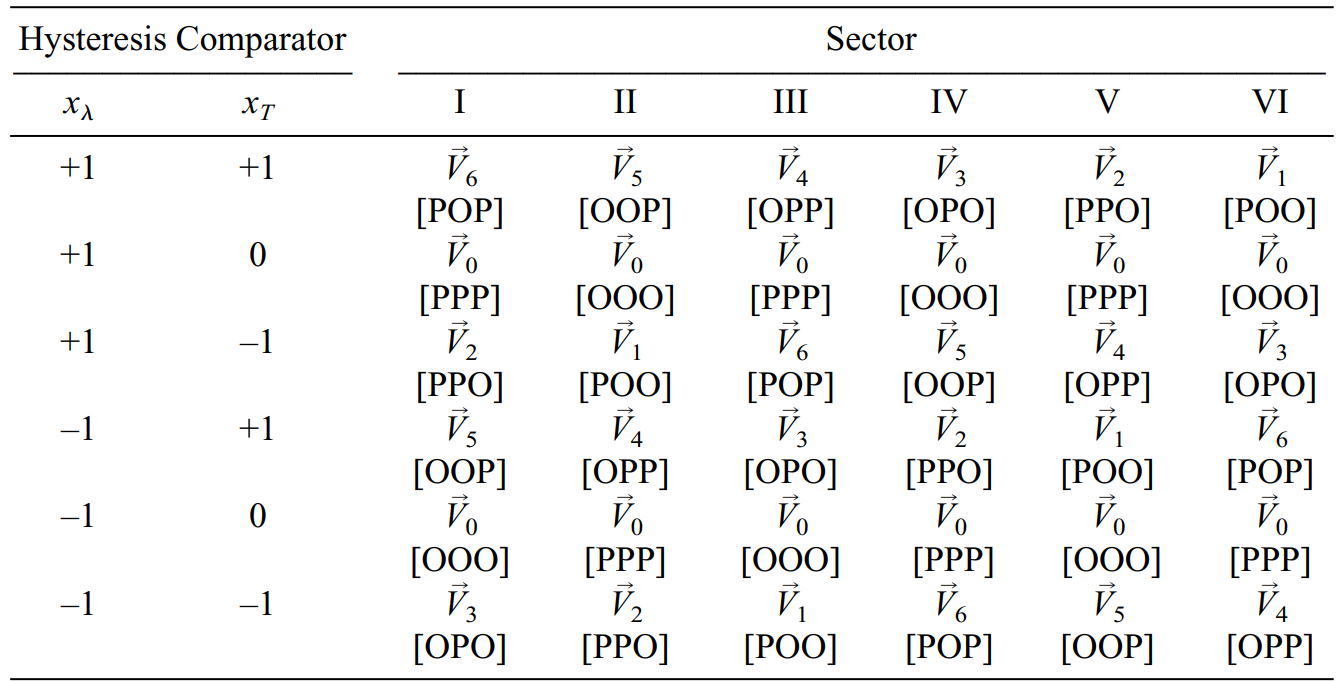
\includegraphics[scale=0.4]{graficos/tabla_14_8_2.png}
\label{tab:14.8-2}
\end{figure}
\FloatBarrier

La lógica de conmutación dada en la Tabla 14.8-1 solo es válida para el motor rotando en sentido antihorario. Cuando el motor opera en sentido horario, se puede usar la lógica de conmutación en la Tabla 14.8-2.

\clearpage
\subsection{Cálculo del Flujo del Estator y el Par}

El vector de flujo del estator $\vec{\lambda_s}$ en el marco estacionario se puede expresar como
\begin{equation}
    \vec{\lambda_s} = \lambda_{ds} + j\lambda_{qs} = \int (v_{ds} - R_s i_{ds}) \, dt + j \int (v_{qs} - R_s i_{qs}) \, dt \tag{14.8-3}
\end{equation}

a partir del cual su magnitud y ángulo son
\begin{equation}
    \lambda_s = \sqrt{\lambda_{ds}^2 + \lambda_{qs}^2} \tag{14.8-4}
\end{equation}
\begin{equation}
    \theta_s = \tan^{-1} \left( \frac{\lambda_{qs}}{\lambda_{ds}} \right) \tag{14.8-5}
\end{equation}
donde $v_{ds}$, $v_{qs}$, $i_{ds}$ e $i_{qs}$ son los voltajes y corrientes del estator medidos. El par electromagnético desarrollado se puede calcular mediante
\begin{equation}
    T_e = \frac{3P}{2} \left( i_{qs} \lambda_{ds} - i_{ds} \lambda_{qs} \right) \tag{14.8-6}
\end{equation}

Las ecuaciones anteriores ilustran que el flujo del estator y el par desarrollado se pueden obtener utilizando los voltajes y corrientes del estator medidos. El único parámetro del motor requerido en los cálculos es la resistencia del estator $R_s`$. Esto contrasta con los esquemas FOC de flujo del rotor directo, donde se necesitan casi todos los parámetros del motor.

\clearpage
\subsection{Simulación del Drive DTC}

\begin{figure}[ht]
\centering
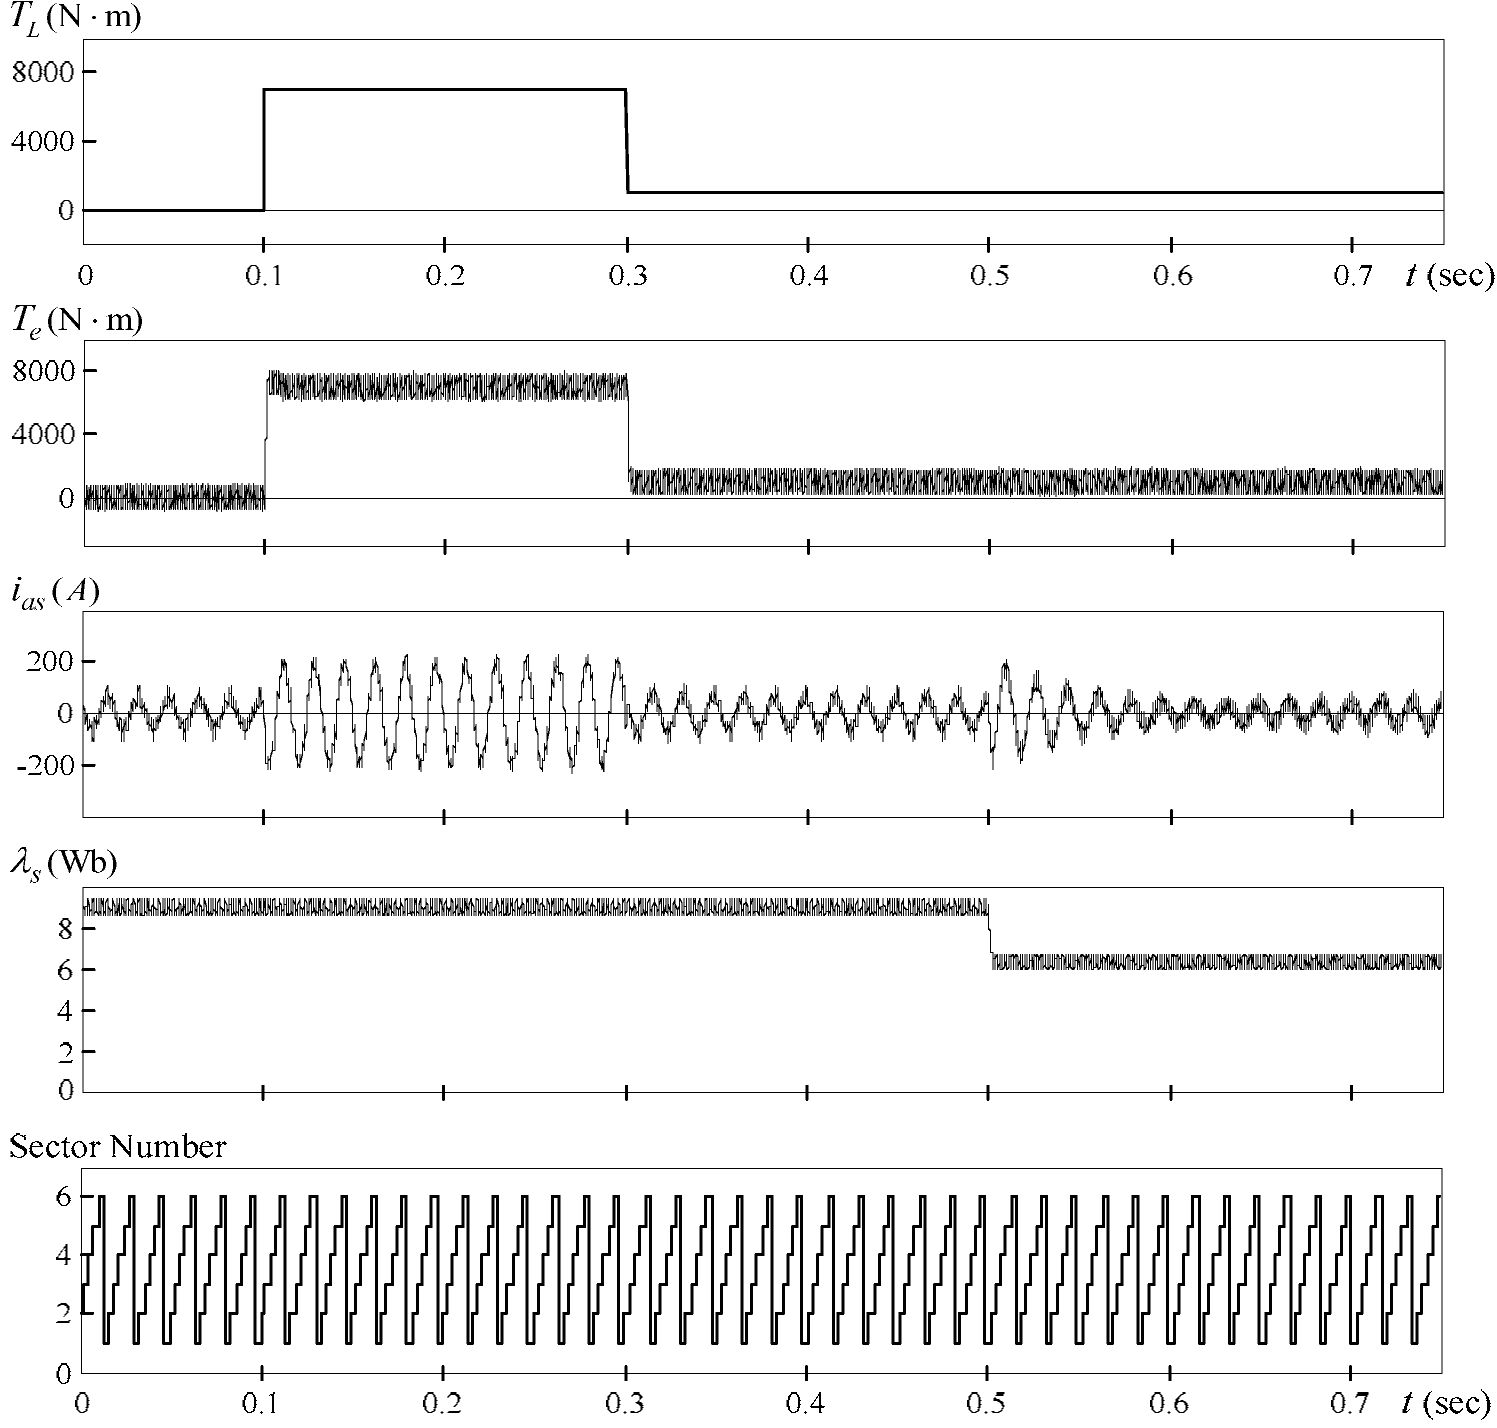
\includegraphics{graficos/img27.jpg}
\caption{Formas de onda simuladas para un drive DTC operando a la velocidad nominal del rotor.}
\label{fig:14.8-5}
\end{figure}
\FloatBarrier

La Figura 14.8-5 muestra las formas de onda simuladas para un drive de motor de inducción utilizando el esquema DTC dado en la Fig. 14.8-2. El lazo de retroalimentación de velocidad del rotor, basado en el cual se genera la referencia de par $T_e^*$, no se muestra para mayor simplicidad. Los parámetros del motor utilizados en la simulación se dan en la Tabla 14.5-1.

Las bandas de tolerancia $\delta_T$ y $\delta_\lambda$ para los comparadores de par y flujo se ajustan de manera que la frecuencia de conmutación promedio $f_{sw}$ de los dispositivos de conmutación sea alrededor de 800 Hz. La referencia de flujo del estator $\lambda_s^*$ se establece en su valor nominal de 9.0 Wb.

El motor opera a la velocidad nominal de $n_r = 1189$ rpm en condiciones de no carga. Suponiendo que el par de carga $T_L$ se incrementa repentinamente a su valor nominal de 7490 N·m en $t = 0.1$ s y luego se reduce a 1000 N·m en $t = 0.3$ s, el par generado $T_e$ responde rápidamente. El rizado de par está determinado por la banda de tolerancia del par $\delta_T$. La corriente del estator $i_{as}$ varía con $T_e$ en consecuencia.

Dado que el flujo del estator $\lambda_s$ y el par del motor $T_e$ se controlan de manera independiente, $\lambda_s$ se mantiene constante durante los cambios repentinos del par de carga. Para demostrar la efectividad del control del flujo del estator, su referencia $\lambda_s^*$ tiene una reducción escalonada desde su valor nominal de 9.0 Wb a 6.3 Wb en $t = 0.5$ s. El flujo del estator $\lambda_s$ responde rápidamente mientras la corriente del estator $i_{as}$ se ajusta en consecuencia para mantener $T_e$ constante. El número de sector obtenido del generador de número de sector en la Fig. 14.8-2 también se muestra en la figura.

\begin{figure}[ht]
\centering
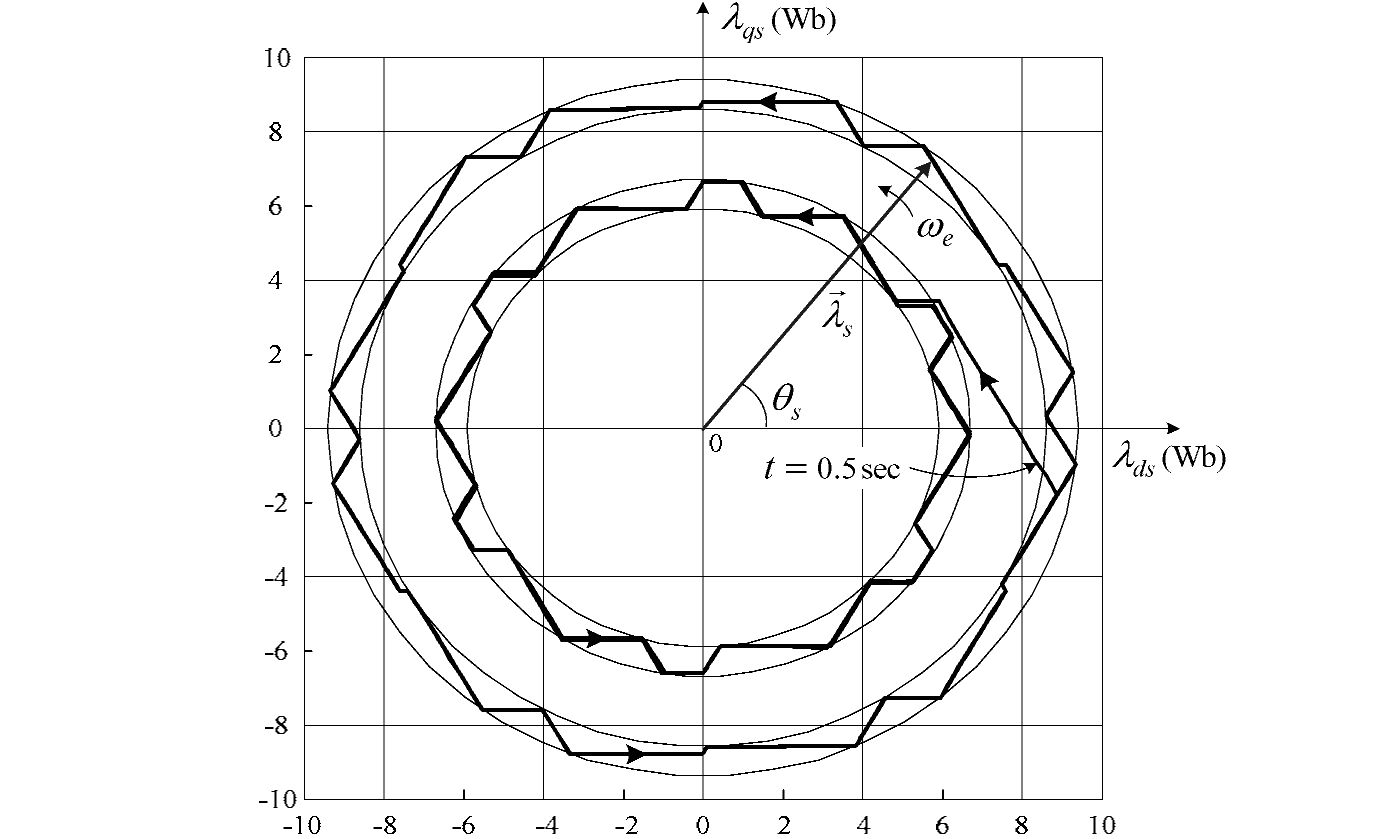
\includegraphics{graficos/img28.jpg}
\caption{Trayectorias del flujo del estator $\lambda_s$ en la Fig. 14.8-5 para $0.35 \leq t \leq 0.75$ s.}
\label{fig:14.8-6}
\end{figure}
\FloatBarrier

La Figura 14.8-6 muestra las trayectorias del flujo del estator $\lambda_s$ en la Fig. 14.8-5 para $0.35 \leq t \leq 0.75$ s. Las trayectorias exterior e interior corresponden a la operación en estado estacionario antes y después de la reducción del flujo del estator en $t = 0.5$ s.

\subsection{Comparación Entre los Esquemas DTC y FOC}

\begin{table}[h]
    \centering
    \caption{Tabla 14.8-3 Comparación Entre los Esquemas DTC y FOC}
    \begin{tabular}{l l l}
        \hline
        \textbf{Comparación} & \textbf{DTC} & \textbf{FOC} \\
        \hline
        Orientación del campo (Transformación & No requerida & Requerida \\
        del marco de referencia) & & \\
        Esquema de control & Simple & Complejo \\
        Control de corriente del estator & No & Sí \\
        Parámetros del motor requeridos & $R_s$ & $R_s$, $L_{ls}$, $L_{lr}$, $L_m$ y $R_r$ \\
        Sensibilidad a las variaciones de los & No muy sensible & Sensible \\
        parámetros del motor & & \\
        Esquema PWM & Banda de histéresis & Basado en portadora, SVM, o \\
        & & banda de histéresis \\
        Comportamiento de conmutación & Variable & Definido (para basado en \\
        & & portadora y SVM) \\
        \hline
    \end{tabular}
    
    \label{table:14.8-3}
\end{table}
\FloatBarrier

Basado en el análisis dado en las secciones anteriores, las características y desventajas de los esquemas DTC y FOC orientado al flujo del rotor se resumen en la Tabla 14.8-3.

\clearpage
\section{RESUMEN}

En este capítulo se presentan los esquemas de control orientado al campo (FOC) y control directo de par (DTC) para drives MV de alto rendimiento. Existen diversos esquemas de control orientado al campo con muchas variaciones y enfoques diferentes. Para facilitar la comprensión del tema, este capítulo se centra en los esquemas de control orientado al flujo del rotor. La otra razón para seleccionar dicho esquema para una discusión detallada radica en su simplicidad y amplia aceptación en la industria de drives. Se elaboran los algoritmos de control para la orientación directa e indirecta del flujo del rotor. Además, se introduce el FOC para drives MV alimentados por CSI. Se discute en detalle el principio operativo del esquema DTC, a partir del cual se proporciona una comparación entre los dos esquemas avanzados.

La implementación de los esquemas FOC y DTC requiere información precisa sobre los parámetros del motor. Sin embargo, los parámetros del motor pueden variar con las condiciones de operación, como el aumento de la temperatura del rotor y la saturación del núcleo magnético. Los problemas relacionados con la sensibilidad de los parámetros y la sintonización de parámetros del motor en línea están fuera del alcance de este libro y, por lo tanto, no se abordan en este capítulo.

\section*{REFERENCIAS}
\footnotesize
\begin{enumerate}
    \item P. C. Krause, O. Wasynczuk, y S. D. Sudhoff, \textit{Analysis of Electric Machines and Drive Systems}, 2ª edición, Wiley-IEEE Press, Nueva York, 2002.
    \item I. Boldear y S. A. Nasar, \textit{Electric Drives}, CRC Press, Boca Ratón, FL, 1999.
    \item D. W. Novotny y T. A. Lipo, \textit{Vector Control and Dynamics of AC Drives}, Clarendon Press, Nueva York, 1996.
    \item P. Vas, \textit{Sensorless Vector and Direct Torque Control}, Oxford University Press, Nueva York, 1998.
    \item J. N. Nash, ``Direct Torque Control, Induction Motor Vector Control Without an Encoder,'' \textit{IEEE Transaction on Industry Applications}, Vol. 33, No. 2, pp. 333--341, 1997.
    \item P. Pohjolainen y C. Stulz, ``Method and Apparatus for Direct Torque Control of a Three-Phase Machine,'' US Patent 5,734,249, 9 páginas, marzo 1998.
    \item S. Heikkila, ``Direct Torque Control Inverter Arrangement,'' US Patent 6,094,364, 13 páginas, julio 2000.
    \item D. Casadei, F. Profumo y A. Tani, ``FOC and DTC: Two Viable Schemes for Induction Motors Torque Control,'' \textit{IEEE Transactions on Power Electronics}, Vol. 17, No. 5, pp. 779--787, 2002.
    \item D. Telford, M. W. Dunnigan y B. W. Williams, ``A Comparison of Vector Control and Direct Torque Control of an Induction Machine,'' \textit{IEEE Power Electronics Specialists Conference (PESC)}, Vol. 1, pp. 421--426, 2000.
\end{enumerate}
\normalsize

\clearpage
\section*{Abreviaturas}
\footnotesize
\begin{flushleft}
\begin{tabular}{ll}
ABB & Asea-Brown-Boveri \\
APOD & Disposición de fase opuesta alternativa \\
CHB & Puente H en cascada \\
CSI & Inversor de fuente de corriente \\
CSR & Rectificador de fuente de corriente \\
DF & Factor de distorsión \\
DPF & Factor de potencia de desplazamiento \\
DTC & Control directo de par \\
ETO & Tiristor de apagado por emisor \\
FC & Controlador de flujo \\
FOC & Control orientado al campo \\
GCT & Tiristor conmutado por compuerta \\
& (también conocido como tiristor conmutado por compuerta integrada) \\
GTO & Tiristor de apagado por compuerta \\
HPF & Filtro de paso alto \\
IEEE & Instituto de Ingenieros Eléctricos y Electrónicos \\
IEGT & Transistor de compuerta mejorada por inyección \\
IGBT & Transistor bipolar de compuerta aislada \\
IPD & Disposición en fase \\
LCI & Inversor conmutado por carga \\
LPF & Filtro de paso bajo \\
MCT & Tiristor controlado por MOS \\
MOSFET & Transistor de efecto de campo de semiconductor de óxido metálico \\
MV & Media tensión (2.3 KV a 13.8 KV) \\
NPC & Punto neutro clamped \\
PCBB & Bloque de construcción de convertidor de potencia \\
PF & Factor de potencia (DF x DPF) \\
PI & Proporcional e integral \\
PLL & Bucle de enganche de fase \\
POD & Disposición de fase opuesta \\
PWM & Modulación por ancho de pulsos \\
pu & Por unidad \\
rms & Valor cuadrático medio \\
rpm & Revoluciones por minuto \\
SCR & Rectificador controlado por silicio (tiristor) \\
SHE & Eliminación selectiva de armónicos \\
SIT & Tiristor de inducción estática \\
SM & Motor síncrono \\
SPWM & Modulación por ancho de pulsos sinusoidal \\
SVM & Modulación por vector espacial \\
THD & Distorsión armónica total \\
TPWM & Modulación por ancho de pulsos trapezoidal \\
VSI & Inversor de fuente de voltaje \\
\end{tabular}
\end{flushleft}
\normalsize

\begin{flushright}
\textit{High-Power Converters and ac Drives. Por Bin Wu}
\newline
© 2006 The Institute of Electrical and Electronics Engineers, Inc.
\end{flushright}

\end{document}